\documentclass[11pt,a4paper,openany]{book}
\usepackage{ctex}
\usepackage{fontenc,xunicode,xltxtra}
\usepackage{changepage}
\usepackage{amsmath,amsthm}
\usepackage{amssymb}
\usepackage{lmodern}
\usepackage{graphicx}
\usepackage{epstopdf}
\usepackage{enumerate}
\usepackage[english]{babel}
\usepackage{amsmath}
\usepackage{amssymb}
\usepackage{latexsym}
\usepackage{multirow}
\usepackage{bigdelim}
\usepackage{color}
\usepackage{graphicx}
\usepackage{wrapfig}
\usepackage{picinpar}
\usepackage{picins}
\usepackage{float}
\usepackage{clrscode}
\usepackage{algorithm} %format of the algorithm
\usepackage{algorithmic} %format of the algorithm
\usepackage{subfigure}
\usepackage{xeCJK}
\usepackage{varwidth}
\usepackage{caption}
\usepackage{lipsum}
\usepackage{framed}
\usepackage[colorlinks]{hyperref}

\setCJKmainfont[BoldFont=SimHei,ItalicFont=KaiTi]{宋体}
\setmonofont{宋体}
\setmainfont{Times New Roman}  %缺省英文字体

\XeTeXlinebreaklocale "zh"   % 针对中文进行断行
\XeTeXlinebreakskip = 0pt plus 1pt minus 0.1pt     % 给予TeX断行一定自由度
%\linespread{1.5}                                  % 1.5倍行距

\newfontfamily{\H}{SimHei}
\newfontfamily{\K}{KaiTi}
\newfontfamily{\S}{黑体}
\setCJKfamilyfont{hwxw}{STXinwei}                    %华文新魏  hwxw
\newcommand{\hwxw}{\CJKfamily{hwxw}}
\setCJKfamilyfont{hei}{SimHei}                       %黑体  hei
\newcommand{\hei}{\CJKfamily{hei}}
\setCJKfamilyfont{song}{SimSun}                      %宋体 song
\newcommand{\song}{\CJKfamily{song}}
\setCJKfamilyfont{kai}{KaiTi}                        %楷体  kai
\newcommand{\kai}{\CJKfamily{kai}}
\setCJKfamilyfont{fs}{FangSong}                      %仿宋 fsong
\newcommand{\fs}{\CJKfamily{fs}}

\newcommand{\xiaosihao}{\fontsize{12pt}{\baselineskip}\selectfont}  %字体大小
\newcommand{\wuhao}{\fontsize{10.5pt}{\baselineskip}\selectfont}

\captionsetup[figure]{name=图}
\captionsetup[table]{name=表}
\definecolor{shadecolor}{rgb}{0.92,0.92,0.92}

%\makeatletter
%\makeatother
\newtheorem{theorem}{\textbf{定理}}[section]
\newtheorem{defination}{\textbf{定义}}[section]
\newtheorem{property}{\textbf{性质}}[section]
\newtheorem{lemma}{\textbf{引理}}[section]
\newtheorem{coro}{\textbf{推论}}[section]
\newtheorem{sample}{\textbf{例}}[section]
\newtheorem{guess}{\textbf{猜想}}[section]
\renewcommand{\figurename}{图}
\floatname{algorithm}{算法}
\newcommand{\reffig}[1]{\textcolor{red}{图}\ref{#1}}

\usepackage{fancyhdr}
\pagestyle{fancy}
\fancyhf{}
\fancyhead[ER]{\rightmark} %奇数页与偶数页分别用字母 O,E 表示
\fancyhead[EL]{\leftmark}
\fancyhead[OL]{\rightmark}
\fancyhead[OR]{\leftmark}
\fancyfoot[LO,RE]{}
\fancyfoot[LE,RO]{-\,\thepage\,-}
\renewcommand{\headrulewidth}{0.4pt}
\renewcommand{\chaptermark}[1]{\markboth{\small 第\,\thechapter\,章\quad #1}{}}
\renewcommand{\sectionmark}[1]{\markright{\small\thesection\quad #1}{}}

\fancypagestyle{plain}{
     \fancyhf{}
     \fancyfoot[LO,RE]{}
     \fancyfoot[LE,RO]{-\,\thepage\,-}
     \renewcommand{\headrulewidth}{0pt}
}
\renewcommand\labelitemi{\ensuremath{\bullet}} % 原来定义为 \textbullet itemsize 黑色圆点
\usepackage{titlesec}
\titleformat{\chapter}{\centering\huge\hei}{第\,\thechapter\,章}{1em}{}[\vspace{-1cm}]
\begin{document}
%\pagestyle{plain}  %取消页码
\chapter{基本概念}
\section{图论概述}
\paragraph{}\textbf{离散数学}是以研究离散量的结构和相互之间的关系为主要目标,其研究对象一般是有限个或可数个元素。离散数学充分契合了计算机科学的特点。离散数学是计算机科学重要的基础理论之一。\\
离散数学主要包括四个方面:数理逻辑、集合论、图论、代数机构。\\
\paragraph{}\textbf{图论[Graph Theory]}是数学的一个分支,它以图为研究对象。\\
\indent 世界上各事物之间,自然界内诸现象之间经常存在着某些必然的联系,需要人们通过研究分析,去揭示这些关系。\\
\indent 人们常把事物、现象用\textcolor[rgb]{1.00,0.00,0.00}{结点}表示,用有向或无向的\textcolor[rgb]{1.00,0.00,0.00}{边}来表示它们之间的联系。这就构成了图论中所讨论的\textcolor[rgb]{1.00,0.00,0.00}{图}。\\
\indent 历史上图论曾经被好多位数学家各自独立地建立过。关于图论的文字记载最早出现在欧拉1736年论著中,其原始问题有很强的实际背景。18世纪在哥尼斯堡城(今俄罗斯加里宁格勒)的普莱格尔河上有7座桥\footnote{在第二章欧拉回路中介绍},将河中的岛屿和河岸连结。\\
\begin{figure}[H]
  \centering
 % \vspace{-10pt}
  \begin{minipage}[!ht]{.35\linewidth}
  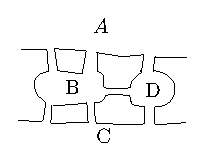
\includegraphics[width=1.0\linewidth]{2_8.eps}
  \caption{哥尼斯堡7桥}
  \end{minipage}
  \begin{minipage}[!ht]{.35\linewidth}
   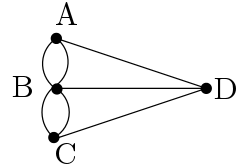
\includegraphics[width=1.0\linewidth]{2.9.png}
  \caption{哥尼斯堡7桥简化}
  \end{minipage}
  %\vspace{0pt}
\end{figure}
\kai{早期的图论与数学游戏有密切的联系:周游世界问题、渡河问题、三家三井问题...20世纪后,图论的应用渗透到其它学科领域,如物理、化学、运筹学、博弈论、计算机网络、社会学、语言学等等。对于基础图论来说,不要求事先掌握高深的数学工具,只需要有集合论和线性代数的基本概念,即可进行学习。}\\

\section{图的基本概念及定义}
\begin{defination}
二元组$G=(V(G),E(G))$称为图。其中$V(G)$是非空集,称为结点集;$E(G)$为$V(G)$各结点之间边的集合,称为边集。\\
\end{defination}
\noindent 常用$G=(V,E)$表示图。\\
当V,E都是有限集合时,称G为\textcolor[rgb]{1.00,0.00,0.00}{有限图}。\\
当V或E是无限集合时,称G为\textcolor[rgb]{1.00,0.00,0.00}{无限图}。\\
一般情况下,给定$G=(V,E)$,如不加特殊说明,认为$V=\{v_1,v_2,v_3,\cdots,v_n\}$,$E=\{e_1,e_2,e_3,\cdots,e_m\}$,即结点数$|V|=n$,边数$|E|=m$。\\
\\
若图中的边为有向的,则称为有向图。\\
若图中的边为无向的,则称为无向图。\\
若图中既有有向边,又有无向边,则称为混合图。\\
\begin{figure}[H]
  \centering
  % Requires \usepackage{graphicx}
  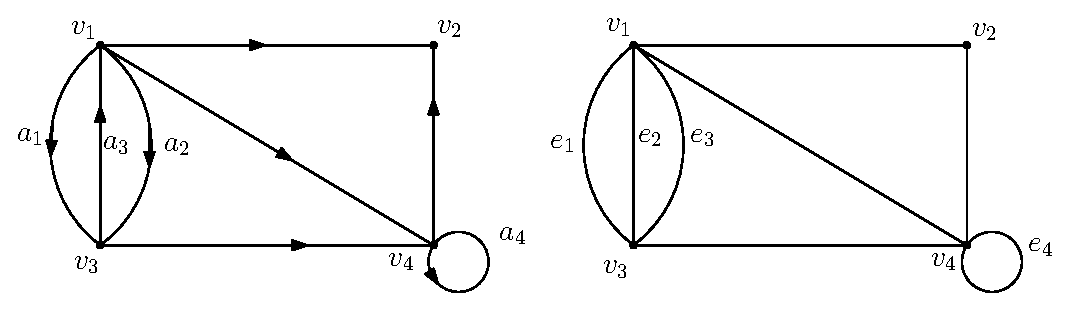
\includegraphics[width=0.9\textwidth]{1_3.eps}\\
  \caption{}
\end{figure}
\noindent 图的边可用$e_k=(v_i,v_j)$表示\\
\vspace{-20pt}
\begin{enumerate}
  \item 称$v_i$与$v_j$是\textcolor[rgb]{1.00,0.00,0.00}{相邻结点}
  \item 称$e_k$分别与$v_i,v_j$\textcolor[rgb]{1.00,0.00,0.00}{相关联}
  \item 如果$e_k$是有向边,称$v_i$是$e_k$的\textcolor[rgb]{1.00,0.00,0.00}{始点},$v_j$是$e_k$的\textcolor[rgb]{1.00,0.00,0.00}{终点},
  并称为$v_i$是$v_j$ 的\textcolor[rgb]{1.00,0.00,0.00}{直接前驱},$v_j$是$v_i$的\textcolor[rgb]{1.00,0.00,0.00}{直接后继}
  \item 如果$e_k$是无向边,称$v_i,v_j$是$e_k$的两个\textcolor[rgb]{1.00,0.00,0.00}{端点}
\end{enumerate}
\begin{defination}
只与一个结点相关联的边称为\textcolor[rgb]{1.00,0.00,0.00}{自环};在同一对结点之间可以存在多条边,称为\textcolor[rgb]{1.00,0.00,0.00}{重边};
含有重边的图叫\textcolor[rgb]{1.00,0.00,0.00}{多重图}。
\end{defination}
\begin{defination}
$G=(V,E)$的某结点所关联的边数称为该结点的度,用$d(v)$表示。如果$V$带有自环,则自环对$d(v)$的贡献为2。\\
有向图中:
\vspace{-15pt}
\begin{itemize}
  \item[-] 以结点V为始点的边数目称为V的正度,记为$d^{+}(v)$
  \item[-] 以结点V为终点的边数目称为V的负度,记为$d^{-}(v)$
\end{itemize}
显然,有$d^{+}(v)+d^{-}(v)=d(v)$
\end{defination}
\begin{defination}
任意两结点间最多只有一条边,且不存在自环的无向图称为\textcolor[rgb]{1.00,0.00,0.00}{简单图}。\\
没有任何边的简单图叫\textcolor[rgb]{1.00,0.00,0.00}{空图},记为$N_n$。\\
任何两结点间都有边的简单图称为\textcolor[rgb]{1.00,0.00,0.00}{完全图}记为$K_n$。($K_n$中每个结点的度为n-1)
\end{defination}
\begin{property}
{设$G=(V,E)$有n个结点,m条边,则}$$\sum_{v\in V(G)}(d_v)=2m$$
\end{property}

\begin{property}
G中度为奇数的结点必为偶数个。
\end{property}
\begin{property}
有向图G中正度之和等于负度之和。
\end{property}
\begin{property}
$K_n$中的边数为$\frac{1}{2}n(n-1)$。
\end{property}
\begin{property}
非空简单图中一定存在度相同的结点。
\end{property}

\begin{defination}
如果图$G=(V,E)$的每条边$e_k=(v_i,v_j)$都赋予一个实数$W_k$做为该边的\textcolor[rgb]{1.00,0.00,0.00}{权},则称G为\textcolor[rgb]{1.00,0.00,0.00}{赋权图}。
如果这些权都是正实数,就称G为\textcolor[rgb]{1.00,0.00,0.00}{正权图}。
\begin{figure}[H]
  \centering
  % Requires \usepackage{graphicx}
  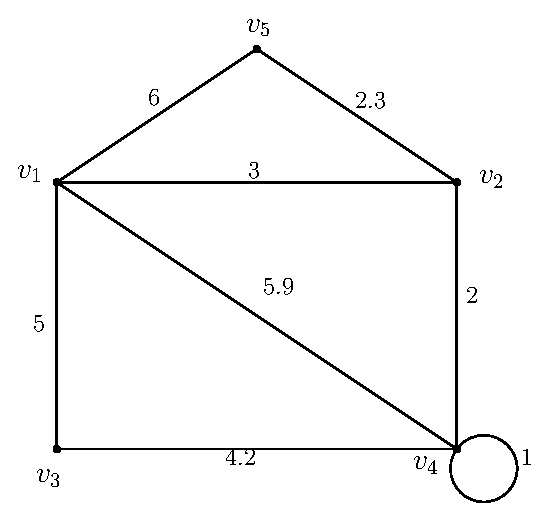
\includegraphics[width=0.5\textwidth]{1_4.eps}\\
  \caption{}
\end{figure}

\end{defination}

\begin{defination}
给定$G=(V,E)$,如果存在另一个图$G'=(V',E')$,满足$V'$包含于V,满足$E'$包含于E,则称$G'$是G的一个\textcolor[rgb]{1.00,0.00,0.00}{子图}。\\
如果$V'=V$,就称$G'$是G的\textcolor[rgb]{1.00,0.00,0.00}{支撑子图}。\\
如果$V'$包含于V,且$E'$包含了在结点子集$V'$之间的所有边,则称$G'$是G的\textcolor[rgb]{1.00,0.00,0.00}{导出子图}。\\
\begin{figure}[H]
  \centering
  % Requires \usepackage{graphicx}
  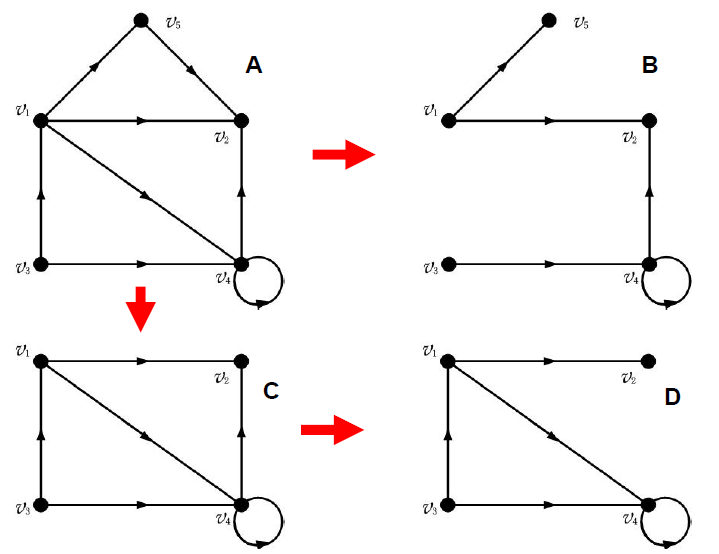
\includegraphics[width=0.8\textwidth]{1.5.png}\\
  \caption{B:支撑子图 C:导出子图 D:子图}
\end{figure}
\end{defination}
\begin{coro}
显然,根据上述的定义,图G是自身的子图,支撑子图,导出子图。\\
\\
空图是图G的支撑子图。\\
\end{coro}
\begin{defination}
称原图G和空图都是图G的\textcolor[rgb]{1.00,0.00,0.00}{平凡子图}。\\
\end{defination}
\begin{defination}
给定两个图$G_1=(V_1,E_1),G_2=(V_2,E_2)$。令
\begin{gather}
  G_1\bigcup G_2=(V_1\bigcup V_2,E_1\bigcup E_2) \\
  G_1\bigcap G_2=(V_1\bigcap V_2,E_1\bigcap E_2)\\
  G_1\bigoplus G_2=(V_1\bigoplus V_2,E_1\bigoplus E_2)
\end{gather}
$1.1,1.2,1.3 $分别称为$G_1$和$G_2$的\textcolor[rgb]{1.00,0.00,0.00}{并}、\textcolor[rgb]{1.00,0.00,0.00}{交}、\textcolor[rgb]{1.00,0.00,0.00}{对称差}。\\
\begin{figure}[H]
  \centering
  % Requires \usepackage{graphicx}
  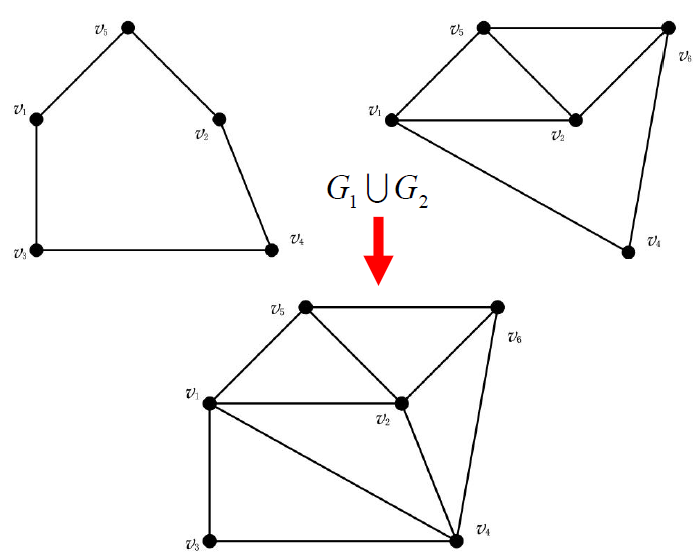
\includegraphics[width=0.8\textwidth]{1.6.1.png}\\
  \caption{$G_1\bigcup G_2$}
\end{figure}
\begin{figure}[H]
  \centering
  % Requires \usepackage{graphicx}
  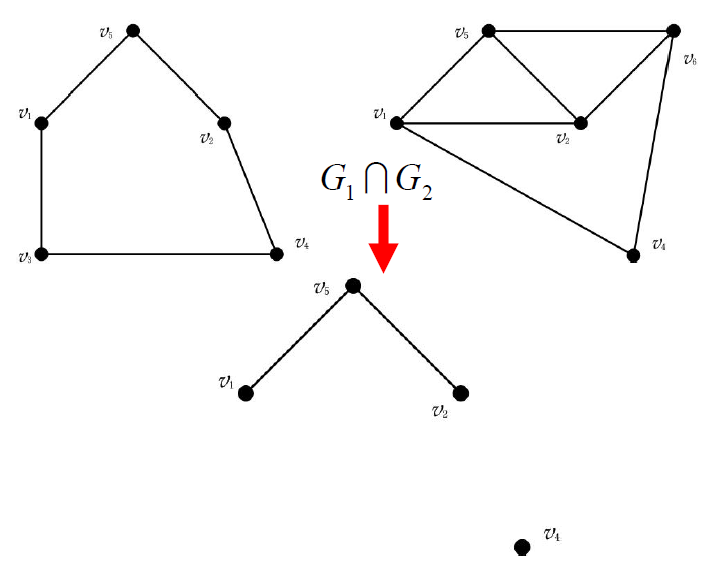
\includegraphics[width=0.8\textwidth]{1.6.2.png}\\
  \caption{$G_1\bigcap G_2$}
\end{figure}
\begin{figure}[H]
  \centering
  % Requires \usepackage{graphicx}
  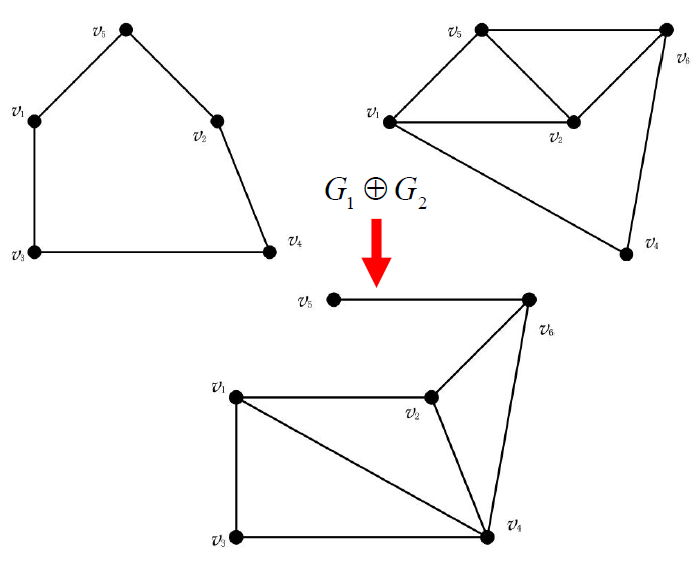
\includegraphics[width=0.8\textwidth]{1.6.3.png}\\
  \caption{$G_1\bigoplus G_2$}\label{fig:163}
\end{figure}
\end{defination}
\song
{
在图G中删掉一个子图H,指删掉H中的各条边,记为\textcolor[rgb]{1.00,0.00,0.00}{$G\quad -\quad H$}。\\
对于简单图G,称$K_n - G$为G的\textcolor[rgb]{1.00,0.00,0.00}{补图},记做\textcolor[rgb]{1.00,0.00,0.00}{$\bar{G}$}。\\
从G中删去某个结点$v$及其关联的边所得到的图记做\textcolor[rgb]{1.00,0.00,0.00}{$G-v$}。\\
从G中删掉某条特定的边e,记做\textcolor[rgb]{1.00,0.00,0.00}{$G-e$}。\\
显然,$G-v$是图G的导出子图,$G-e$是图G的支撑子图。\\
}
\begin{defination}
如G为无向图,则$$\Gamma(v)=\{u|(v,u)\in E\}$$称为v的\textcolor[rgb]{1.00,0.00,0.00}{邻点集}。\\
如G为有向图,v是其中一个结点,则$$\Gamma^{+}(v)=\{u|(v,u)\in E\}$$称为v的直接后继或者\textcolor[rgb]{1.00,0.00,0.00}{外邻集};相应的
$$\Gamma^{-}(v)=\{u|(v,u)\in E\}$$称为v的直接前趋集或内邻集。\\
\end{defination}

\begin{defination}
两个图$G_1=(V_1,E_1),G_2=(V_2,E_2)$,如果$V_1$,$V_2$之间存在双射$f$,而且$(u,v)\in E_1$,当且仅当$(f(u),f(v))\in E_2$时,称$G_1$和$G_2$\textcolor[rgb]{1.00,0.00,0.00}{同构}。记做$$G_1\cong G_2$$\\
\end{defination}
\begin{shaded}
\noindent 从定义知,若$G_1\cong G_2$,必须满足:\\
(1)$|V(G_1)|=|V(G_2)|$,$|E(G_1)|=|E(G_2)|$\\
(2)$G_1$和$G_2$结点度的非增序列相同\\
(3)$G_1$和$G_2$存在同构的导出子图\\
\end{shaded}
{\xiaosihao\hwxw 思考:如何判定两图同构?}\\
\begin{figure}[H]
  \centering
  % Requires \usepackage{graphicx}
  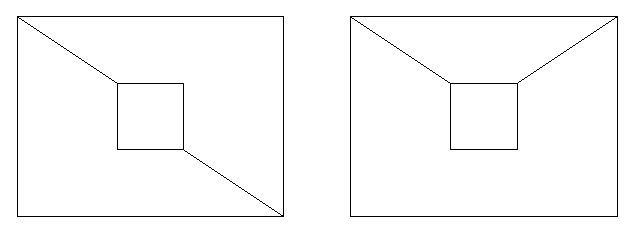
\includegraphics[width=0.8\textwidth]{tonggou.eps}\\
  \caption*{}
\end{figure}
\section{图的代数表示}
图在计算机中如何表示(拓扑结构、边权值...)?如何对图进行描述或运算?所以我们需要用代数的方法来描述图!\\
\begin{defination}
表示了结点间的邻接关系的矩阵称为\textcolor{red}{邻接矩阵}。\\
\end{defination}
\begin{shaded}
\noindent 有向图的邻接矩阵$\mathbf{A}$是一个n 阶方针,其元素为:
$$\mathbf{A}=[a_{ij}]_{n\times n} \quad a_{ij}=\begin{cases}
        1& (v_i,v_j)\in E\\
        0& others
    \end{cases}$$
\end{shaded}
\begin{figure}[H]
  \centering
  % Requires \usepackage{graphicx}
  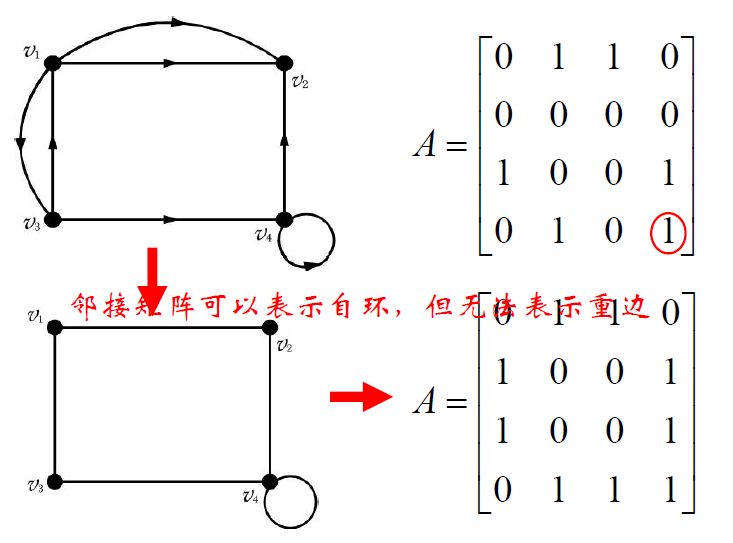
\includegraphics[width=0.8\textwidth]{1.9.png}\\
  \caption{}
\end{figure}
\textcolor{red}{权矩阵:}赋权图常用权矩阵A进行表示。
\begin{shaded}
其元素为:
$$\mathbf{A}=[a_{ij}]_{n\times n} \quad a_{ij}=\begin{cases}
        w_{ij}& (v_i,v_j)\in E\\
        0& others
    \end{cases}$$
\end{shaded}
\begin{figure}[H]
  \centering
  % Requires \usepackage{graphicx}
  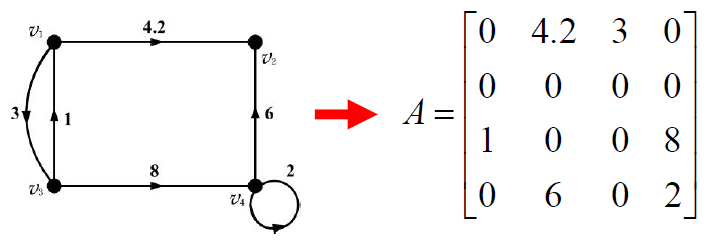
\includegraphics[width=0.8\textwidth]{1.10.png}\\
  \caption{}
\end{figure}
\textcolor{red}{关联矩阵:}关联矩阵表示结点与边之间的关联关系。\\
\begin{shaded}
有向图G的关联矩阵$\mathbf{B}$是$n\times m$的矩阵,当给定结点和边的编号之后,其元素
$$\mathbf{B}=[b_{ij}]_{n \times m} \quad b_{ij}=
\begin{cases}
        1& e_j=(v_i,v_k)\in E\\
        -1& e_j=(v_k,v_i)\in E\\
        0& others
    \end{cases}
$$
\end{shaded}
\begin{figure}[H]
  \centering
  % Requires \usepackage{graphicx}
  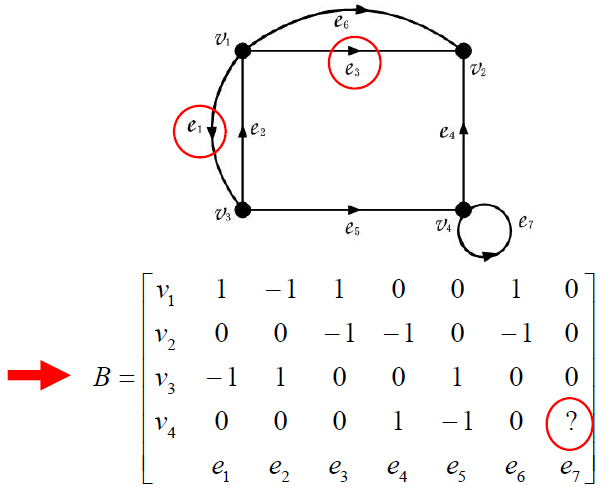
\includegraphics[width=0.8\textwidth]{1.11.png}\\
  \caption{}
\end{figure}
\begin{shaded}
无向图G的关联矩阵$\mathbf{B}$是$n\times m$的矩阵,当给定结点和边的编号之后,其元素
$$\mathbf{B}=[b_{ij}]_{n \times m} \quad b_{ij}=
\begin{cases}
        1& e_j \text{与}v_i\text{关联}\\
        0& others
    \end{cases}
$$
\end{shaded}
\begin{figure}[H]
  \centering
  % Requires \usepackage{graphicx}
  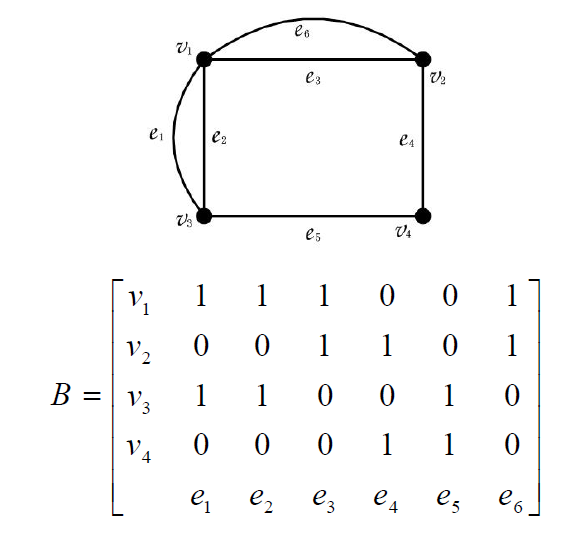
\includegraphics[width=0.8\textwidth]{1.12.png}\\
  \caption{}
\end{figure}
\begin{shaded}
\noindent 关联矩阵的性质(有向图):\\
(1)每列只有两个非零元:1、-1\\
(2)第$i$行非零元的数目恰为结点$v_i$的度,其中1的数目为其正度,-1的数目为其负度\\
关联矩阵的性质(无向图):\\
(1)每列只有一个非零元:1\\
(2)第i行1的数目恰为结点$v_i$的度\\
\textbf{关联矩阵能够表示重边,但不能表示自环。}
\end{shaded}

\textcolor{red}{邻接矩阵、权矩阵、关联矩阵可以表示重边,但无法表示自环}\\
邻接矩阵、权矩阵、关联矩阵的优点是一旦写出代数表达式,则可得到确定图,且非常直观。缺点是(1)不能表示自环(2)在计算机上存储邻接矩阵与关联矩阵时,将占据较大的存储空间并可能增加计算复杂度。所以需要引入\textbf{边列表}、\textbf{正向表}、\textbf{逆向表}、\textbf{邻接表}。\\
\noindent \textbf{边列表}由两个m维向量A和B组成。若$e_k=(v_i,v_j)$,则$$A(k)=i,B(k)=j$$
如果G为赋权图,则再增加一个m维变量Z,若$e_k$的权值为$w_k$,则令$$Z(k)=w_k$$
如图1.13所示是边列表,边列表的实质是关联矩阵的压缩形式并克服了其缺点。\\
\begin{figure}[H]
  \centering
  % Requires \usepackage{graphicx}
  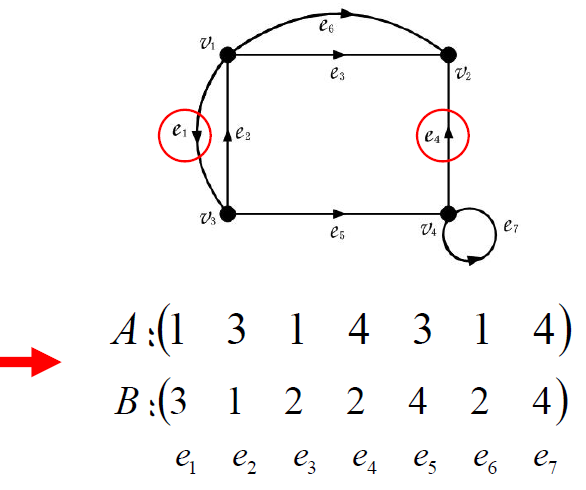
\includegraphics[width=0.8\textwidth]{1.13.png}\\
  \caption{}
\end{figure}
\indent 赋权图只需增加权值向量,如果G是赋权图,则再增加一个m维向量Z,若$e_k$的权是$w_k$,则令$Z(k)=w_k$。例如图1.14的边列表形式是:
\begin{align}
  A:( & 4 \quad 4 \quad 1 \quad 2\quad 2 \quad 2 \quad 4)\\
  B:( & 1 \quad 1 \quad 2 \quad 2 \quad 4 \quad 3 \quad 3)\\
  Z:(&  5 \quad 3 \quad 4 \quad 6 \quad 7 \quad 2 \quad 4)
\end{align}
\begin{figure}[H]
  \centering
  % Requires \usepackage{graphicx}
  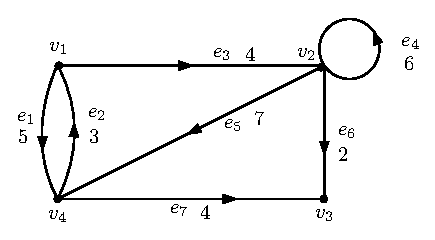
\includegraphics[width=0.6\textwidth]{1_14.eps}\\
  \caption{}
\end{figure}
类似的可以得到无向图的边列表。\\
\noindent \textbf{正向表}:当对G的结点与边进行编号后,正向表将每个节点的直接后继集中在一起存放。\\
\indent \textcolor{red}{有向图的正向表}由一个$(n+1)$维向量A,一个m维向量B组成。$A(i)$表示结点$v_i$的第一个后继在B中的地址,
B中存放这些后继结点的编号,$A(n+1)=m+1$。\\
\indent 对赋权图,用m维向量Z存放权,$Z(k)=w_k$。\\
有向图正向表如图1.15所示:\\
\begin{figure}[H]
  \centering
  % Requires \usepackage{graphicx}
  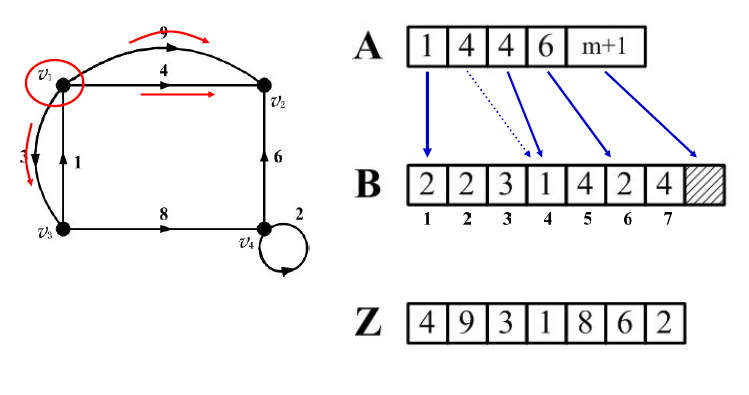
\includegraphics[width=0.8\textwidth]{1.15.png}\\
  \caption{}
\end{figure}
\begin{shaded}
正向表存在下述关系:\\
1.$d^{+}(v_i)=A(i+1)-A(i)$\\
2. $A(i)=\sum^{i-1}_{j=1}d^{+}(v_j)+1$\\
3.从$B(A(i))$到$B(A(i+1)-1)$的任意一个值,都是$v_i$的直接后继。
\end{shaded}

\textcolor{red}{无向图的正向表结构:}\\
B向量中存放的是相应邻结点的编号,因此为2m维。相应地,Z向量也变成2m维。\\
无向图正向表如图1.16所示:\\
\begin{figure}[H]
  \centering
  % Requires \usepackage{graphicx}
  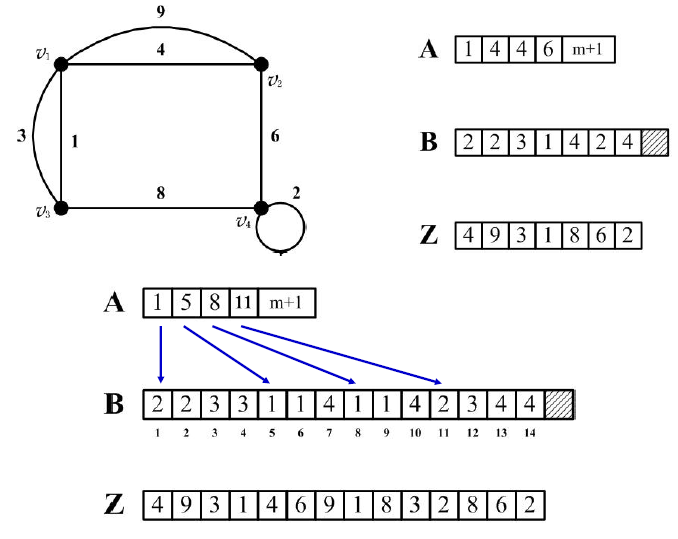
\includegraphics[width=0.8\textwidth]{1.16.png}\\
  \caption{}
\end{figure}
\textcolor{red}{逆向表}:与正向表相反,逆向表是将每个结点的直接前趋集中在一起存放。\\
逆向表实质是对有向图邻接矩阵的列进行压缩的结果。\\
{\hwxw 思考:正(逆向表优缺点是什么?)}\\
例如图1.14的逆向表是:\\
\begin{figure}[H]
  \centering
  % Requires \usepackage{graphicx}
  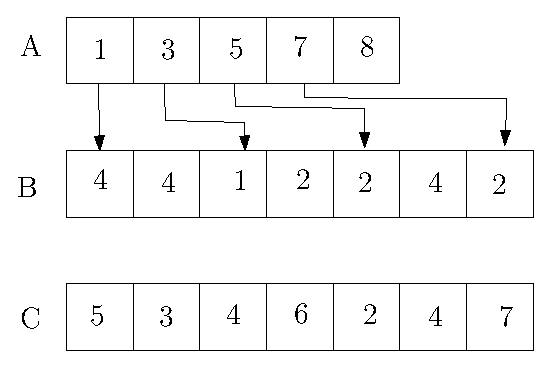
\includegraphics[width=0.6\textwidth]{1_17.eps}\\
  \caption*{}
\end{figure}
\textcolor{red}{邻接表}:采用单链表结构表示一个图。其中基本单元为表结点,如下所示:\\
\begin{figure}[H]
  \centering
  % Requires \usepackage{graphicx}
  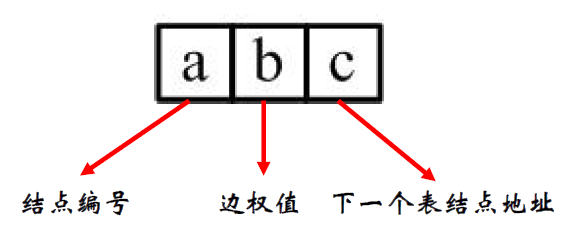
\includegraphics[width=0.8\textwidth]{1.17.1.png}\\
  \caption*{}
\end{figure}
\begin{figure}[H]
  \centering
  % Requires \usepackage{graphicx}
  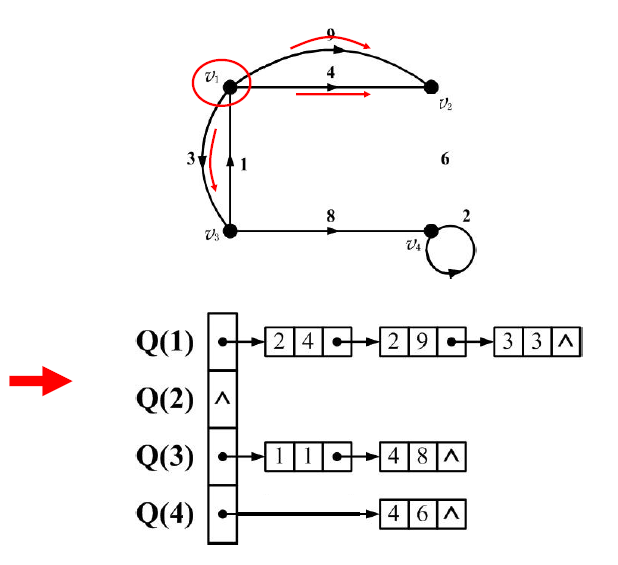
\includegraphics[width=0.9\textwidth]{1.18.png}\\
  \caption*{}
\end{figure}

\chapter{道路与回路}
\section{道路与回路}
\begin{defination}\K 有向图G=(V,E)中,若边序列P=($e_{i1},e_{i2},\dots,e_{iq}$ ),其中$e_{ik}=(v_l,v_j )$ 满足$v_l$ 是$e_{ik-1}$ 的终点,$v_j$是$e_{ik+1}$的始点,就称P 是G 的一条\textbf{有向道路}。\\ 如果$e_{iq}$的终点也是$e_{i1}$的始点,则称P 是G的一条\textbf{有向回路}。
\end{defination}
\begin{figure}[H]
  \centering
  % Requires \usepackage{graphicx}
  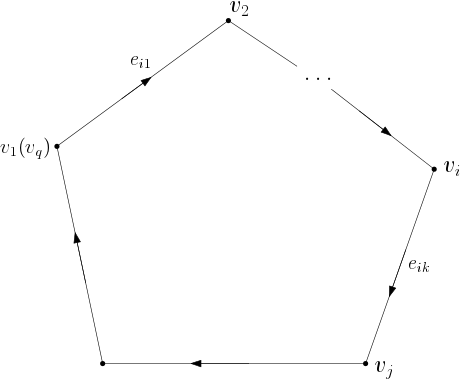
\includegraphics[width=0.5\textwidth]{2.1.1.png}\\
  \caption*{一条有向的回路}
\end{figure}

\begin{sample}\H 下图中,边序列($e_5,e_4,e_5,e_7$ )是有向道路,($e_5,e_4,e_5,e_7,e_3$ )是有向回路。\\
($e_5,e_4,e_1,e_2$ ) 是简单有向道路,($e_5,e_4,e_1,e_2,e_3$ ) 是简单有向回路。\\
($e_1,e_2$ )是初级有向道路,($e_1,e_2,e_3$ )是初级有向回路。
\begin{figure}[H]
  \centering
  % Requires \usepackage{graphicx}
  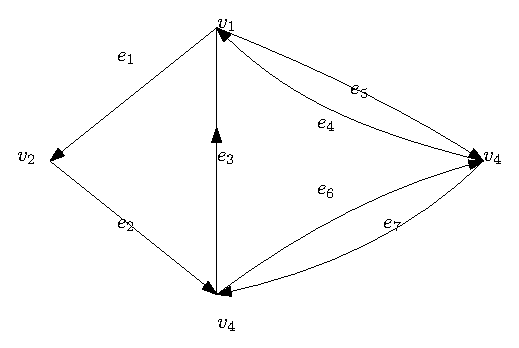
\includegraphics[width=0.5\textwidth]{2_1.eps}\\
\caption{}\label{fig:2.1}
\end{figure}
\end{sample}
\begin{defination}\K
无向图G=(V,E)中,若点边交替序列P=$(v_{i1},e_{i1},v_{i2},e_{i2},\dots,e_{iq-1},v_{iq} )$满足$v_{ik}$,$v_{ik+1}$是$e_{ik}$ 的两个端点,则称P是G 中的一条链或道路。\\
\\
如果$v_{iq}=v_{i1}$,则称P 是G 中的一个圈或\textbf{回路}。\\
\noindent 如果P中没有重复出现的边,称之为\textbf{简单道路}或\textbf{简单回路},若其中结点也不重复,又称之为\textbf{初级道路}或\textbf{初级回路}。
\end{defination}
\textbf{思考}非初级有向道路的简单有向道路有什么特征?
\begin{sample}\H
下图中边序列:\\
($e_4,e_5,e_4,e_6$ )是道路;\\
($e_4,e_5,e_4,e_6,e_3$ )是回路;\\
($e_4,e_5,e_1,e_2$ )是简单道路,($e_4,e_5,e_1,e_2,e_3$ ) 是简单回路;\\
($e_1,e_2$ )是初级道路,($e_1,e_2,e_3$ ) 是初级回路。
\begin{figure}[H]
  \centering
  % Requires \usepackage{graphicx}
  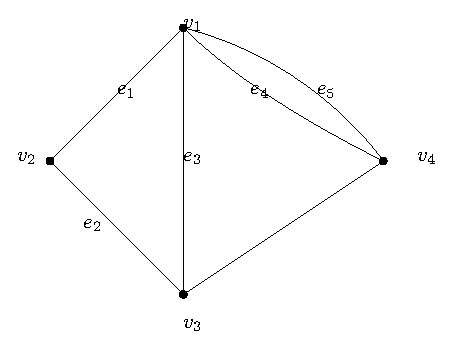
\includegraphics[width=0.5\textwidth]{2_2.eps}\\
\caption{}\label{fig:2.2}
\end{figure}
\end{sample}
\begin{sample}
\H 设C是简单图G中含结点数大于3的一个初级回路,如果结点$v_i$和$v_j$在C中不相邻,而边($v_i,v_j$ )∈E(G),则称($v_i,v_j $) 是C的一条弦。\\
若对每一个$v_k∈V(G)$,都有d($v_k$ )≥3,则G中必含带弦的回路。
\begin{adjustwidth}{0.62cm}{0.62cm}
\textbf{证明:}\S {在G中构造一条极长的初级道路$P=(e_{i1},e_{i2},\dots,e_{iq} )$\\
不妨设$e_{i1}=(v_0,v_1 )$,$e_{il}=(v_{l-1},v_l )$。\\
由于P是极长的初级道路,所以$v_0$ 和$v_1$ 的邻接点都在该道路P上。\\
由已知条件,d($v_0$ )≥3,不妨设$\Gamma(v_0$ )={$v_1,v_{ij},v_{ik},\dots$}。 其中1<j<k;\\
这时($v_0,v_1,\dots,v_{i},v_0$ )是一条初级回路,而($v_0,v_{ij}$ ) 就是该回路中的一条弦。}
 \end{adjustwidth}
\end{sample}
% 改编到教材11页
\begin{sample}\H
设C是简单图G中含结点数大于3的一个初级回路;\\
如果结点$v_i$和$v_j$在C中不相邻,而边($v_i,v_j$ )∈E(G),则称($v_i,v_j$ ) 是C 的一条弦。\\
若对每一个$v_k$∈V(G),都有d($v_k$)≥3,则G 中必含带弦的回路。
\begin{adjustwidth}{0.62cm}{0.62cm}
\textbf{证明 :}\\
 在G中构造一条极长的初级道路P=($e_{i1},e_{i2},\dots,e_{iq}$ ),不妨设$e_{i1}$=($v_0,v_1$ ),$e_{il}=(v_{l-1},v_l $)。\\
 由于P是极长的初级道路,所以$v_0$ 和$v_1$ 的邻接点都在该道路P上。\\
 由已知条件,d($v_0$)≥3,不妨设$\Gamma(v_0$)={$v_1,v_{ij},v_{ik},\dots$},其中1<j<k;\\
 这时($v_0,v_1,\dots,v_{ik},v_0$ ) 是一条初级回路,而($v_0,v_{ij}$ ) 就是该回路中的一条弦。\\
\end{adjustwidth}
\end{sample}
\begin{sample}\H{
设G=(V,E)是无向图,如果V(G)可以划分为子集X和Y,使得对所有的e=(u,v)∈E(G),u和v都分属于X和Y,则称G是二分图。\\
证明:如果二分图G中存在回路,则它们都是由偶数条边组成的。\\}
\begin{adjustwidth}{0.62cm}{0.62cm}
\textbf{证明:}\\
设C是二分图G的任一回路,不妨设$v_0$∈X是C的始点,由于G是二分图, 所以沿回路C 必须经过偶数条边才能达到某结点$v_i$∈X,因而只有经过偶数边才能回到$v_0$。\\
\end{adjustwidth}
\end{sample}
\begin{defination}\H
 设G是无向图,若G的任意两结点之间都存在道路,就称G是\textbf{连通图},否则称为\textbf{非连通图}。\\
 如果G是有向图,不考虑其边的方向,即视之为\textbf{无向图},若它是连通的,则称G是连通图。\\
若连通子图H不是G的任何连通子图的真子图,则称H是G的\textbf{极大连通子图},或称\textbf{连通支}。显然G的每个连通支都是它的\textbf{导出子图}。
\end{defination}
\begin{sample}\K
图2.1和图2.2都是连通图,图2.3是非连通图。\\
其中(a)有两个连通支, 它们的结点集分别是{$v_1,v_2,v_3$ }和{$v_4,v_5$ };\\
(b)有三个连通支,其结点集是{$v_1,v_2,v_3$ },{$v_4,v_5$ } 和{$v_6$ }。\\
\end{sample}
\begin{figure}
  \centering
  \begin{minipage}[!ht]{.6\linewidth}
  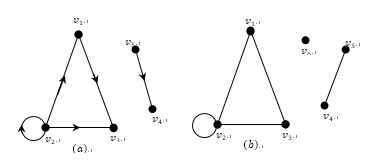
\includegraphics[width=1.0\linewidth]{2.3.png}
  \caption{}
  \end{minipage}
  \begin{minipage}[!ht]{.4\linewidth}
   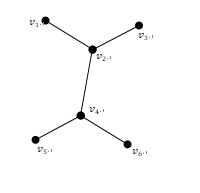
\includegraphics[width=1.0\linewidth]{2.4.png}
  \caption{}
  \end{minipage}
\end{figure}
\begin{sample}\K
图2.4是连通图,它不含回路,而且在任意两结点之间都只有唯一的一条初级道路。这种图称为树,它是含边数最少的连通图。
\end{sample}
\begin{sample}\K
设G是简单图,证明当$m=\frac{1}{2}(n-1)(n-2)$时,G是连通图。\\
\begin{adjustwidth}{0.62cm}{0.62cm}
\textbf{证明:}\\
假定G是非连通图,则至少含有2个连通支。\\
设分别为$G_1=(V_1,E_1)$,$G_2=(V_2,E_2)$。\\
其中$|V_1 (G_1 )|=n_1$,$|V_2 (G_2 )|=n_2$,$n_1+n_2=n$。\\
由于G 是简单图,因此$$|E_1 (G_1 )|\leq\frac{1}{2} n_1(n_1-1)$$$$|E_2 (G_2 )|\leq\frac{1}{2}n_2 (n_2-1)$$$$m\leq\frac{1}{2} n_1(n_1-1)+\frac{1}{2}n_2(n_2-1)$$\\
由于$n_1$≤n-1,$n_2$≤n-1,\\
所以$$m\leq\frac{1}{2}(n-1)(n_1-1+n_2-1)$$$$=\frac{1}{2}(n-1)(n-2)$$\\
与已知条件矛盾,故G是连通图。\\
\end{adjustwidth}
\end{sample}

\section{道路与回路的判定}
\paragraph{}通常可以利用邻接矩阵或搜索法判定某个图G的两结点间是否存在道路,或者判定它是否连通。首先介绍\textbf{ 邻接矩阵}的判定方法。
\paragraph{}设$A=(a_{ij})_{n\times n}$是G的邻接矩阵。由A的定义,$a_{ij}=1$表示$(v_i,v_j )\in E(G)$,即$v_i$可以通过某条边e到达$v_j$,者说G中有道路从$v_i$到$v_j$。根据矩阵乘法,设$A^2=(a_{ij}^{(2)})$,有
\begin{displaymath}
a_{ij}^{(2)}=\sum_{k=1}^{n}a_{ik}.a_{kj}
\end{displaymath}
$a_{ij}^{(2)}\neq 0$当且仅当存在k,使$a_{ik}=a_{kj}=1$。也就是说,如果G中存在结点$v_k$,满足$(v_i,v_k )$,$(v_i,v_k )\in E(G)$,即经过2 条边$(v_i,v_k)$,$(v_k,v_j)$,$v_i$可以到达$v_j$时,$a_{ij}^{(2)}\neq 0$。 同理,$A^l(l≤n)$中的元素$a_{ij}^{(l)}\neq0$表示了$v_i$ 可以经过$l$条边到达$v_j$。因此令$$P=A+A_2+\cdots+A_n,$$如果$p_{ij}=t$,说明$v_i$有t条道路可以到达$v_j$。若$p_{ij}=0$,即n步之内$v_i$不能到达$v_j$,则在G中不存在$v_i$到$v_j$ 的路。否则,若$v_i$ 经过$l(l>n)$步可达$v_j$,由\textbf{抽屉原理},该道路上一定存在重复出现的结点$v_k$,而$v_k$之间的这段路C 是一个回路。删去这段回路$v_i$ 仍然可达$v_j$。 由于G 中只存在n个不同的结点,所以只要$v_i$有道路到$v_j$,一定有$p_{ij}≠0$。
\paragraph{}在许多实际问题中,往往只要求了解$v_i$与$v_j$之间是否存在道路。对此可以采用逻辑运算的方法,即$$a_{ij}^{(l)}=\bigvee_{k=1}^{n}(a_{ik}^{(l-1)}\bigwedge a_{ij}),l=2,3,\cdots,n。$$相应地,$$P=A\bigvee A^2 \bigvee \cdots \bigvee A^n$$就是图G 的道路矩阵。
\paragraph{}用上述方法求G的道路矩阵,计算复杂性为Ο($n^4$ )。以下介绍的Warshall算法是一个更好的方法,其计算复杂性是Ο($n^3$)。
\begin{adjustwidth}{0.62cm}{0.62cm}
\textbf{Warshall算法}\\
begin\\
\begin{enumerate}
\item $P\leftarrow A$,
\item for i=1 to n do
\item \quad for j=1 to n do
\item \qquad for k=1 to n do\\ \indent\quad$p_{jk}\leftarrow p_{jk}\bigvee(p_{jk}\bigwedge p_{ik})$。
\end{enumerate}
\end{adjustwidth}
\begin{sample}\K
采用Warshall算法计算图2.5道路矩阵的过程是:\\
$P\leftarrow
\begin{bmatrix}
0&1&1&0&0\\
0&0&1&1&0\\
0&0&0&0&1\\
0&0&0&0&0\\
1&0&0&1&0\\
\end{bmatrix}
$\\
$P(i=1)=\begin{bmatrix}
0&1&1&0&0\\
0&0&1&1&0\\
0&0&0&0&1\\
0&0&0&0&0\\
1&1&1&1&0\\
\end{bmatrix}\quad P(i=2)= \begin{bmatrix}
0&1&1&1&0\\
0&0&1&1&0\\
0&0&0&0&1\\
0&0&0&0&0\\
1&1&1&1&0\\
\end{bmatrix}
$\\
$P(i=3)=\begin{bmatrix}
0&1&1&1&1\\
0&0&1&1&1\\
0&0&0&0&1\\
0&0&0&0&0\\
1&1&1&1&1\\
\end{bmatrix}\quad P(i=4)=P(i=3),
$\\
\begin{figure}[h]
\vspace{-50pt}
\parbox[t]{0.5\textwidth}{$
P(i=5)=\begin{bmatrix}
1&1&1&1&1\\
1&1&1&1&1\\
1&1&1&1&1\\
0&0&0&0&0\\
1&1&1&1&1\\
\end{bmatrix}$}
\centering
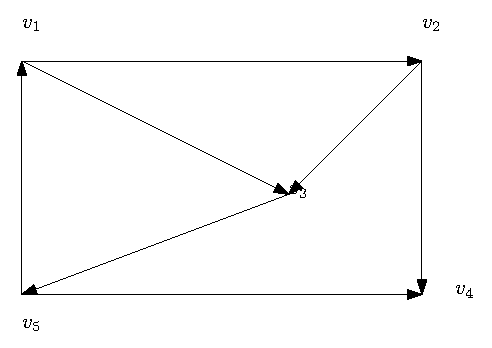
\includegraphics[width=0.4\textwidth]{2_5.eps}%
\captionsetup{margin=3em}
\caption{}
\vspace{-30pt}
\end{figure}
\end{sample}
\begin{theorem}Warshall算法的结果是图G的道路矩阵。\\
\K \textbf{证明:}该定理的严格证明需要对三层循环分别使用归纳法。现只证其最外层循环。\\
基始:当i=1时,\\
$p_{jk}^{(l)}=p_{jk}\bigvee (p_{jl}\bigwedge p_{lk}),\quad k=1,2,\cdots,n, \quad j=1,2,\cdots,n$;\\
$p_{jk}^{(1)}=1$当且仅当$p_{jk}=1$或$p_{j1}=p_{1k}=1$,其中$p_{jk}=1$表明$v_j$直接可达$v_k$,\\
$p_{j1}=p_{1k}=1$表明$v_j$直接经过$v_1$ 可达$v_k$。\\
因此$p_{jk}^{(l) }=1$ 当且仅当结点集{$v_j,v_1,v_k$ } 之间有$v_j$到$v_k$的路。\\
 \indent i=2时,$p_{jk}^{(2)}=p_{jk}^{(1)}\bigvee(p_{j2}^{(1)}∧p_{2k}^{(1)})$,$k=1,2,\cdots,n$,\quad $j=1,2,\cdots,n$。\\
 $p_{jk}^{(2)}=1$当且仅当$p_{jk}^{(1)}=1$ 或$ p_{j2}^{(1)}=p_{2k}^{(1)} =1$,其中$p_{jk}^{(1)}=1$表明结点集{$v_j,v_1,v_k$ }之间有$v_j$到$v_k$的道路;\\$p_{j2}^{(1)} $和$p_{2k}^{(1)}$为1 表明{$v_j,v_1,v_2,v_k $} 之间$v_j$有必通过$v_2$到达$v_k$的道路。\\
 因此,$p_{jk}^{(2)}=1$ 当且仅当结点集{$v_j,v_1,v_2,v_k $} 中有$v_j$到$v_k$ 的道路。\\
\indent 设i=n-1时,$p_{jk}^{(n-1)}=1$当且仅当结点集{$v_j,v_1,v_2,\cdots,v_{n-1},v_k$}之中有$v_j$到$v_k$的道路。\\
\indent 则i=n时,$p_{jk}^{(n)}=p_{jk}^{(n-1)}\bigvee(p_{jn}^{(n-1)}\bigwedge p_{nk}^{(n-1)}),k=1,2,\cdots,n,\quad j=1,2,\cdots,n$。\\由归纳假设,$p_{jk}^{(n-1)}=1 $ 表明结点集{$v_j,v_1,v_2,\cdots,v_{n-1},v_k$ }中有$v_j$到$v_k$的路;\\
$p_{jn}^{(n-1)}=p_{nk}^{(n-1)}=1$表明结点集{$v_j,v_1,v_2,\cdots,v_{n-1},v_k$ }中$v_j$有通过$v_n$ 到达$v_k$ 的道路。\\
因此,$p_{jk}^{(n)}=1$即是结点集{$v_j,v_1,\cdots,v_n,v_k $}之中有$v_j$ 到$v_k$ 的道路。\\
\end{theorem}
\indent 采用搜索的方法判断G中某一结点$v_0$到另一结点$v_j$是否存在道路经常更加方便。常用的搜索法有广探法(Breadth First Search) 和深探法(Depth First Search)。
\\ \indent \textbf{广探法(BFS)}是从G的任一结点$v_0$开始, 找它的直接后继集$Γ^+ (v_0)$,记为$A_1$,然后对$A_1$中的每一结点分别找它们的直接后继集,这些直接后继集的并记为$A_2$。 依此类推,直至达到目的。为了避免结点的重复搜索,可以首先对全部结点都给一个标记“0”,当$v_i$ 被搜索到时,如果其标记为0,则$v_i$进入直接后继集,同时标记改为1,否则由于$v_i$ 已被搜索因此不再进入直接后继集。
% 改编到14页
\begin{sample}
用BFS方法找图2.6中$v_1$到$v_4$的一条道路。\\
\begin{figure}[!ht]
  \centering
  % Requires \usepackage{graphicx}
  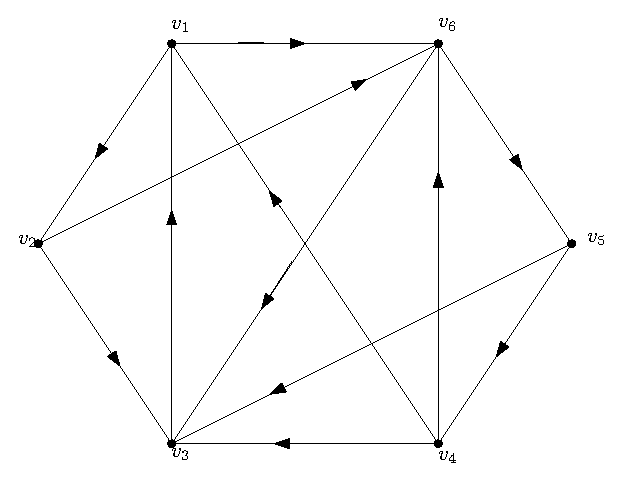
\includegraphics[width=0.8\textwidth]{2_6.eps}\\
  \caption{}\label{fig:2.6}
\end{figure}
\textbf{解:}如果采用正向表的输入结构,则有\\
\begin{figure}[h]
  \centering
   \vspace{-10pt}
  % Requires \usepackage{graphicx}
  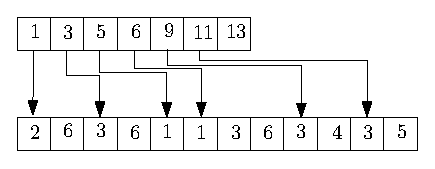
\includegraphics[width=0.8\textwidth]{2_6BFS.eps}\\
  \caption*{}\label{} \vspace{-40pt}
\end{figure}
$\because \Gamma^{+}(v_1)={v_2,v_6}$\\
$\therefore A_1={v_2,v_6}$。\\
$\because \Gamma^{+}(v_2)={v_3,v_6}$\\
$\Gamma^{+}(v_6)={v_3,v_5}$\\
$\therefore A_2={v_3,v_5}$。\\
$\because  \Gamma^{+}(v_3)={v_1},\Gamma^{+}(v_5)={v_3,v_4}$,\\
$\therefore A_3={v_4}$\\
\indent 从上例中可知,用BFS方法求两点间道路的计算复杂性是O(m)。
\end{sample}
\begin{figure}[h]
  \centering
  \vspace{-10pt}
  % Requires \usepackage{graphicx}
  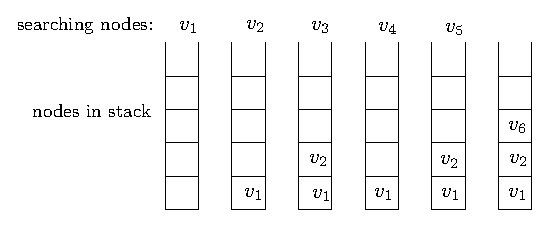
\includegraphics[width=0.8\textwidth]{2_6DFS.eps}
  \caption{}\label{fig:2.7}\vspace{-10pt}
\end{figure}
\indent \textbf{深探法(DFS)}的特点与BFS截然不同。它从某一结点$v_0$开始,只查找$v_0$的某个直接后继$v_1$,记下$v_1$ 的父亲$v_0$,然后再找$v_1$的某个未搜索过的直接后继$v_2$。 依此类推。当从某个结点$v_j$无法再向下搜索时,退回到它的父亲$v_{j-1}$,然后再找$v_{j-1}$的另一个未查过的直接后继。形象地说,DFS的特点是尽量向下搜索,只有碰壁才回头。\\
\indent 采用栈结构以及前述的标记结点的方法可以完成DFS的搜索过程。\\
\begin{sample}\K
用DFS方法找图2.6中$v_1$到$v_4$的一条道路。\\
 \textbf{解:}\\
 数据输入依然采用正向表。\\
 $v_1$的第一个直接后继是$v_2,v_1$进栈;\\
 $v_2$的第一个后继是 $v_3,v_2$进栈。\\
 $v_3$的后继是$v_1$,但已标记,故退栈。\\
 $v_2$的另一个后继是$v_6$,$v_2$进栈;\\
 $v_6$的第1 个后继是已标记结点$v_3$,第2个后继是$v_5$,$v_6$进栈。\\
 $v_5$ 的后继是$v_4$。\\
 至此,已搜索到$v_1$到$v_4$的一条道路。\\
 整个搜索过程可用图2.7 形象地表示。其计算复杂性也是O(m)。
\end{sample}
\section{欧拉道路与回路}
\subsection{欧拉道路的引入}
\indent 1736年瑞士著名数学家欧拉(Leonhard Euler)发表了图论的第一篇论文“哥尼斯堡七桥问题”。这个问题是这样的:哥尼斯堡城被Pregel 河分成了4 部分,它们之间有7 座桥。如图2.8 所示。当时人们提出了一个问题,能否从城市的某处出发,过每座桥一次且仅一次最后回到原处。欧拉的文章漂亮地解决了这个问题。他把4块陆地设想为4 个结点,分别用A、B、C、D 表示,而将桥画成相应的边,如图2.9。于是问题转化为在该图中是否存在经过每条边一次且仅一次的回路。欧拉的论文给出了解决这类问题的准则,并对七桥问题给出了否定的结论。\\
\begin{figure}[H]
  \centering
  % Requires \usepackage{graphicx}
  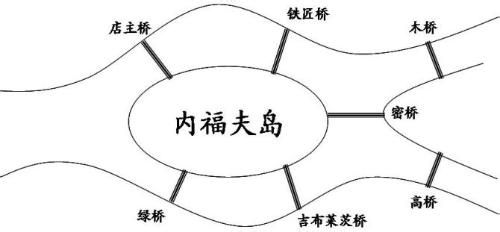
\includegraphics[width=0.5\textwidth]{2.3.1.jpg}
  \caption*{哥尼斯堡七桥}
\end{figure}
\begin{figure}[h]
  \centering
  \vspace{-10pt}
  \begin{minipage}[!ht]{.35\linewidth}
  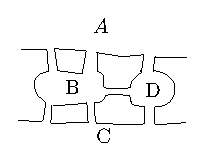
\includegraphics[width=1.0\linewidth]{2_8.eps}
  \caption{}
  \end{minipage}
  \begin{minipage}[!ht]{.35\linewidth}
   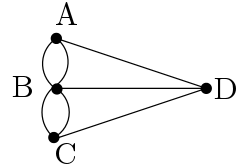
\includegraphics[width=1.0\linewidth]{2.9.png}
  \caption{}
  \end{minipage}
  \vspace{-25pt}
\end{figure}
\begin{defination}\K
给定无孤立结点的无向图G,经过图G每边一次且仅一次的迹称为\textbf{欧拉路}。无向连通图G=(V,E)中的一条经过所有边的简单回路(道路)称为G 的\textbf{欧拉回路(道路)}。
\end{defination}
\begin{theorem}\H
无向连通图G存在欧拉回路的充要条件是G中各结点的度都是偶数。\\
\textbf{证明:}\\
必要性。若G中有欧拉回路C,则C过每一条边一次且仅一次。对任一结点v来说,如果C经由$e_i$进入v,则一定通过另一条边$e_j$ 从v 离开。因此结点v的度是偶数。\\
充分性。由于G是有穷图,因此可以断定,从G的任一结点$v_0$出发一定存在G的一条简单回路C。这是因为各结点的度都是偶数,所以这条简单道路不可能停留在$v_0$以外的某个结点,而不能再向前伸延以至构成回路C。\\
如果E(G)=C,则C就是欧拉回路,充分性得证。\\
否则在G中删去C的各边,得到$G_1=G-C$。$G_1$可能是非连通图,但每个结点的度保持为偶数。这时,$G_1$中一定存在某个度非零的结点$v_i$,同时$v_i$也是C中的结点。否则C的结点与$G_1$的结点之间无边相连,与G是连通图矛盾。\\
同样理由,从$v_i$ 出发,$G_1$中$v_i$ 所在的连通支内存在一条简单回路$C_1$。 显然$C\bigcup C_1$ 仍然是G的一条简单回路,但它包括的边数比C 多。\\
继续以上构造方法,最终有简单回路$C'=C\bigcup C_1\bigcup\cdots\bigcup C_k$,它包含了G的全部边,即C' 是G 的一条欧拉回路。\\
以上采用了构造性证明的方法,即证明过程本身就给出了问题求解的步骤。\\
\end{theorem}
\begin{sample}\K
试找出图2.10的一条欧拉回路。
\end{sample}
\begin{figure}[h]
  \centering
  % Requires \usepackage{graphicx}
  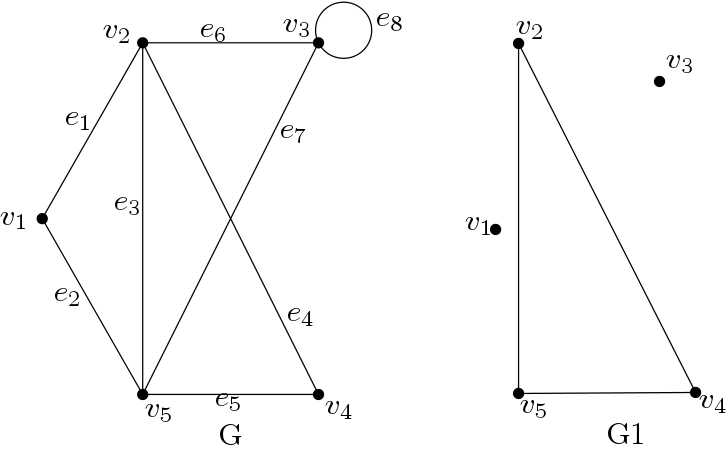
\includegraphics[width=0.9\textwidth]{2.10.png}\\
  \caption{}
\end{figure}
\indent 解:从任一点,比如$v_1$开始,可构造简单回路$C=(e_1,e_6,e_8,e_7,e_2)$。$G_1  =G-C$中的$v_2,v_5$度非零且是C中的结点,从$v_2$ 开始$G_1$中有简单回路$C1=(e_3,e_5,e_4)$。 因此 $C\bigcup C_1=(e_1,e_3,e_5,e_4,e_6,e_8,e_7,e_2)$ 包含了G的所有边,即是G的一条欧拉回路。
\begin{coro}
无向连通图G中只有2个度为奇的结点,则G存在欧拉道路。\\
\textbf{证明:}设$v_i$和$v_j$是两个度为奇数的结点。作$G'=G+(v_i,v_j)$,则G'中各点的度都是偶数。由定理2.3.1,G'有欧拉回路,它包含边$(v_i,v_j)$,删去该边,得到一条从$v_i$到$v_j$的简单道路,它恰好经过了G的所有边,亦即是一条欧拉道路。
\end{coro}
\begin{coro}\K
若有向连通图G中各结点的正、负度相等,则G存在有向欧拉回路。\\
其证明与定理2.3.1的证明相仿。
\end{coro}
\begin{sample}
七桥问题中既不存在欧拉回路也不存在欧拉道路。
\end{sample}
\begin{sample}\K
 设连通图G=(V,E)有k个度为奇数的结点,证明E(G)可以划分成$\frac{k}{2}$条简单道路。\\
 \textbf{证明:}由性质1.1.2,k是偶数。在这k个结点间增添k/2条边,使每个结点都与其中一条边关联,得到$G'$,$G'$中各结点的度都为偶数。\\
 由定理2.3.1,$G'$中有欧拉回路C,这$\frac{k}{2}$条边都在C 上且不相邻接。删去这些边,得到k/2条简单道路,它们包含了G的所有边。亦即E(G)划分成了$\frac{k}{2}$ 条简单道路。\\
 \end{sample}
\begin{sample}\K
下图中,图$G1$是欧拉图;\\
图$G2$不是欧拉图,但$G2$中存在欧拉路;\\
图$G3$中即不存在欧拉回路,也不存在欧拉路。\\
\begin{figure}[h]
  \centering
  % Requires \usepackage{graphicx}
  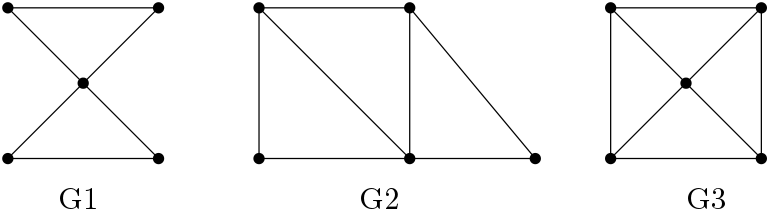
\includegraphics[width=0.8\textwidth]{2.f1.png}\\
  \caption*{}
\end{figure}
\end{sample}
\begin{sample}\K
下图中,图$D1$中既不存在有向欧拉回路,也不存在有向欧拉路;\\
图$D2$是欧拉图;\\
图$D3$不是欧拉图,但$D3$中存在有向欧拉路。\\
\begin{figure}[h]
  \centering
  % Requires \usepackage{graphicx}
  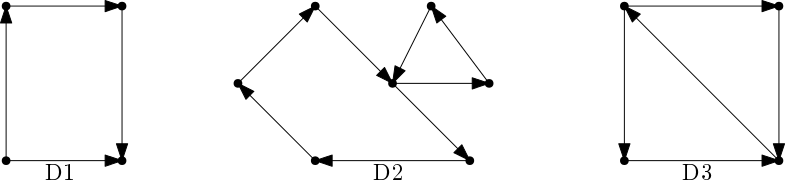
\includegraphics[width=0.8\textwidth]{2.f2.png}\\
  \caption*{}
\end{figure}
\end{sample}
\begin{sample}\K
蚂蚁比赛问题:甲,乙两只蚂蚁分别位于2.11图中的节点a,b处,并设图中的边长度是相等的。甲乙进行比赛:从它们所在的结点出发,走过图中的所有边,最后到达结点c 处。如果它们的速度相同,问谁先到达目的地?\\
\begin{figure}[h]
  \centering
  \vspace{0pt}
  % Requires \usepackage{graphicx}
  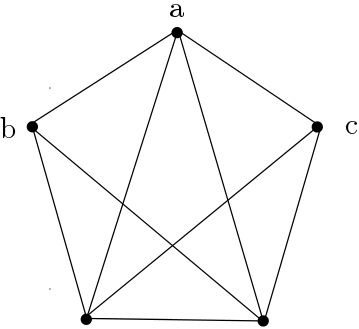
\includegraphics[width=0.3\textwidth]{mayi.png}
  \caption{}
\end{figure}
\textbf{解:}在图中仅有两个度数为奇数的结点b,c因而存在从b到c的欧拉通路,蚂蚁乙走到c只要一条欧拉通路,边数为9条。而蚂蚁甲要走完所有的边到达c,至少要先走一条边到达b,再走一条欧拉通路,因而它至少要走10条边才能到达c,所以乙必胜。
\end{sample}
\begin{sample}
一个编码盘分成16个相等的扇面,每个扇面分别由绝缘体和导体组成,可表示0和1两种状态,其中a,b,c,d四个位置的扇面组成一组二进制输出,如图2.12所示。试问这16个二进制数的序列应如何排列,才恰好能组成0000到1111的16组四位二进制输出,同时旋转一周后又返回到0000状态?\\
\begin{figure}[h]
  \centering
  \vspace{-10pt}
  \begin{minipage}[!ht]{.35\linewidth}
  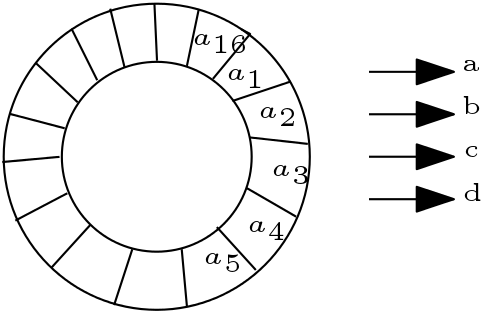
\includegraphics[width=1.0\linewidth]{2.11.png}
  \caption{}
  \end{minipage}
  \begin{minipage}[!ht]{.6\linewidth}
   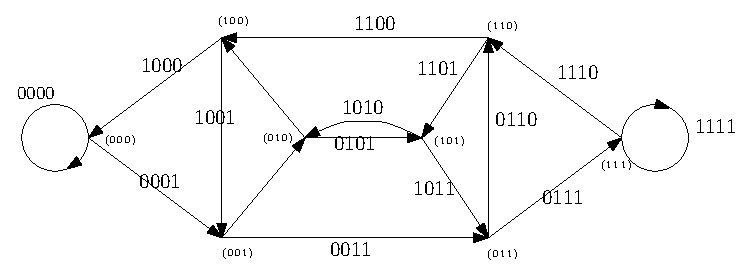
\includegraphics[width=1.0\linewidth]{2_12.eps}
  \caption{}
  \end{minipage}
  \vspace{-20pt}
\end{figure}
\textbf{解:}我们发现如果从状态$a_1 a_2 a_3 a_4 (a_i=0或1)$逆时针方向旋转一个扇面,那么新的输出是$a_2 a_3 a_4 a_5$,其中有三位数字不变。因此可以用8个结点表示从000 到111 这8 个二进制数。这样从结点($a_{i-1} a_i a_{i+1}$)可以到达结点($a_i a_{i+1} 0$)或($a_i a_{i+1} 1$),其输出分别为($a_{i-1} a_i a_{i+1} 0$)和($a_{i-1} a_i a_{i+1} 1$),这样可以得到图2.13。它是有向连通图,共有16 条边,且每结点的正、负度相等。由推论2.3.2,它存在有向欧拉回路。其中任一条都是原问题的解,比如(0000101001101111)就是一种方案。\\
\end{sample}
\subsection{科学家的故事-莱昂哈德$\centerdot$欧拉}
\indent 莱昂哈德$\centerdot$欧拉(Leonhard Euler ,1707 年4 月15 日~ 1783 年9 月18 日),瑞士数学家、自然科学家。1707 年4 月15 日出生于瑞士的巴塞尔,1783 年9 月18 日于俄国圣彼得堡去世。欧拉出生于牧师家庭,自幼受父亲的影响。13 岁时入读巴塞尔大学,15 岁大学毕业,16 岁获得硕士学位。\\
\indent 欧拉是18 世纪数学界最杰出的人物之一,他不但为数学界作出贡献,更把整个数学推至物理的领域。他是数学史上最多产的数学家,平均每年写出八百多页的论文,还写了大量的力学、分析学、几何学、变分法等的课本,《无穷小分析引论》、《微分学原理》、《积分学原理》等都成为数学界中的经典著作。在几何方面,欧拉解决了哥尼斯堡七桥问题,成为图论、拓扑学的滥觞。欧拉对数学的研究如此之广泛,因此在许多数学的分支中也可经常见到以他的名字命名的重要常数、公式和定理。\\
\indent 此外欧拉还涉及建筑学、弹道学、航海学等领域。\\
\begin{figure}[h]
  \centering
  % Requires \usepackage{graphicx}
  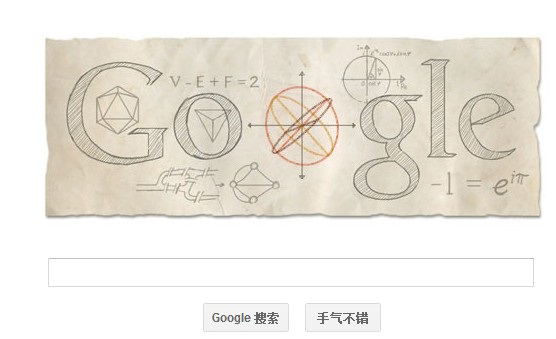
\includegraphics[width=0.6\textwidth]{oula1.png}
\end{figure}
\indent 2013 年4 月15 日是欧拉诞辰的306 周年,谷歌更换了首页涂鸦向这位数学天才致敬。在那天的谷歌涂鸦中,融入了许多欧拉的数学成就。

\section{哈密尔顿回路}
\subsection{哈密尔顿回路的引入} 一个包含一个无向图中所有的点的初级回路被称作\textbf{哈密尔顿回路}(Hamilton Cycle)。这源于1857 年Sir William Hamilton 发明的一种游戏——遍历一个正十二面体,不能经过一个点两次。一个含有哈密尔顿回路的图称作\textbf{哈密尔顿图}(Hamiltonian)。 事实上,在哈密尔顿之前,1759年,欧拉就已经研究了在一个国际象棋棋盘上骑士的遍历问题(Knight's Tour on a Chess Board)(图a给出了一个解)。如果我们对旅行商问题再加上一重限制,两个城市之间的旅行费用只有$1$ 和$\infty$ (也就是说不可能经过这条边),那么这个TSP问题就变成了这个图中所有的旅行费用为1 的边中是否存在一条哈密尔顿回路。然而,直到现在,即使这种TSP 问题的特殊情况仍然没有解决:没有有效算法构造图中的哈密尔顿回路,虽然是否真的有这样的算法也不知道。\\
\begin{figure}[H]
\centering
\subfigure[骑士遍历问题的一个解]{
\label{Fig.sub.h1}
\includegraphics[width=0.3\textwidth]{图0.png}}
\subfigure[正十二面体的一个哈密尔顿回路]{
\label{Fig.sub.h2}
\includegraphics[width=0.3\textwidth]{图1.png}}
\subfigure[赫歇尔图]{
\label{Fig.sub.h3}
\includegraphics[width=0.3\textwidth]{图2.png}}
\caption{正十二面体图(图b)是一个哈密尔顿图,而赫歇尔图(图c)则不是}
\label{Fig.lable}
\end{figure}
但是,边不交哈密尔顿回路问题现在我们已经可以很容易解决,这个问题在如下的例子中给出。\\
\begin{sample} {\K 约翰得到了n($\geq 2$)种宝石,他想把这n种宝石串成几条n-长的项链(每条项链中都含有每种宝石一颗),他希望自己串成的每条项链都本质不同,请问他最多能串出几条项链。两条项链\textbf{本质不同},当且仅当每种宝石相邻的宝石种类都不同。}\end{sample}
\textbf{解} 我们第一步估算上界:将n种宝石记作$v_0,v_1,v_2,\dots,v_{n-1}$, 作完全图$K_n$, 则此题转化为计算完全图$K_n$ 中边不交H 回路计数问题;完全图中一共有$C_{n}^{2}=\frac{n(n-1)}{2}$条边,每条H回路长为n,所以至多存在$[\frac{C_n^2}{n}]=[\frac{n-1}{2}]$ 条边不交H回路。
\\第二步可以构造一个解。\\
$n=2k+1$时,如下图(Figure 2)将$v_1,v_2,\dots,v_{2k}$,排列在一个圆上,将$v_0$放在圆心。联结$(v_0,v_1,v_2,v_{2k},v_3,v_{2k-1},\dots,v_{k-1},v_{k+3},v_{k},v_{k+2},v_{k+1},v_0)$形成一条H回路;删除联结线,下面将$v_1,v_2,\dots,v_{2k}$命名为顺时针下一个点的名字,也即,将$v_{2k-1}$命名为$v_{2k}$,$v_{2k}$命名为$v_1$,$v_1$命名为$v_2$,$v_2$命名为$v_3$;重复执行联结操作,这样就得到k条边不交H回路。\\
$n=2k+2$时,$2\mid k$时,将$v_{2k+1}$插入$v_{\frac{k+2}{2}}$和$v_{\frac{3k+2}{2}}$的边中;$2 \nmid k$ 时,将$v_{2k+1}$ 插入$v_{\frac{k+3}{2}}$ 和$v_{\frac{3k+3}{2}}$的边中;依次就可以构造出k条边不交H回路。
综上,约翰可以串出$[\frac{n-1}{2}]$条本质不同的项链。
\begin{figure}[h]
 \centering
  % Requires \usepackage{graphicx}
  \includegraphics[width=0.5\textwidth]{图3.png}
  \caption{一种构造方案}\label{Fig.label}
\end{figure}

\begin{theorem} {\K $n\geq 2$的完全图$K_n$可以被分解成边不交哈密尔顿回路。}\end{theorem}
\begin{proof} 直接参照上例即可。 \end{proof}

\section{哈密尔顿回路的几个重要判定定理}
\begin{theorem} {\K 对于阶大于3的连通图G,能够满足$$\forall x, y \in G \wedge (x,y) \notin G \Rightarrow d(x)+d(y)\geq k$$
如果$k=n$那么G就是一个哈密尔顿图,而如果$k<n$那么G中就含有一条k-长路,以及一个长度至少为$\frac{k+2}{2}$ 的回路。}\end{theorem}
\begin{proof} 假设G不是哈密尔顿图,我们找到G中的最长道路P($=x_1x_2\dots x_l$)。由于P是最长道路,所以P是极长道路。考虑$$\Gamma(x_1)=\{x_j|(x_1, x_j) \in G\}, \Gamma^{+}(x_l)=\{x_{j+1}|(x_j, x_l) \in G\}.$$
我们可以断言这两个集合是不交的。否则就会产生回路,进而与G的连通性和非哈密尔顿图的性质违,这点留给读者自己证明。
那么由定理中的不等式,我们有$$k \leq d(x_1)+d(x_l)=\#\Gamma(x_1)+\#\Gamma^{+}(x_2)\leq l-1 \leq n-1.$$$\#S$ 表示集合S 的大小。
如果$k=n$,现在就已经产生了矛盾,G是一个哈密尔顿图。如果$k<n$,那么G中就存在一条长度为$l-1=k$的路。
如果再考虑$x_1$和$x_l$度的关系,不妨$d(x_l)>d(x_1)$,也即$d(x_l)\geq\frac{k}{2}$,我们就能够找到一个长度至少为$\frac{k+2}{2}$ 的回路了。\end{proof}

\begin{defination} \K 若$v_i$和$v_j$是简单图G的不相邻结点,且满足$d(v_i)+d(v_j)\geq k$,那么在G中增加边$(v_i, v_j)$,重复这个过程,直到不再有这样的结点对为止。最终得到的图称为G 的k-闭包,记作$C_k(G)$。\end{defination}

\begin{coro} \K 如果$\delta(G)\geq \frac{n}{2}$,那么图$G$是哈密尔顿图。\end{coro}

\begin{theorem} \K 图G是哈密尔顿图,当且仅当$C_n(G)$是;图G有哈密尔顿路,当且仅当$C_{n-1}(G)$有。\end{theorem}
\begin{proof} 这是\textbf{定理 0.2.1}的简单推论。\end{proof}

下面介绍一个中国数学家范更华给出的一个充分性判定条件。

\begin{theorem}[范更华]\K 对于一个2-连通图,如果对于任意一对距离为2的结点$x, y, d(x,y)=2$,都有$$max\{d(x),d(y)\}\geq \frac{n}{2},$$ 那么$G$是哈密尔顿图。\end{theorem}
\begin{proof}略\end{proof}

再介绍一个非常实用的平面图具有哈密尔顿圈的必要条件。(尽管我们还没有严谨地定义过平面图)
\begin{theorem}[Kozyrev and Grinberg] \K 如果一个平面图含有哈密尔顿圈$C$,用$f_k,g_k$表示$C$内部和外部的k 边形的数量,我们有$$\sum_{k\geq3}(k-2)(f_k-g_k)=0.$$\end{theorem}
这个定理可以很方便地证明一类平面图的非哈密尔顿性。

\begin{sample}[Grinberg图] Figure 3不含哈密尔顿回路。\end{sample}
\begin{proof} Figure 3中只有五边形、八边形和九边形。$$3(f_5-g_5)+6(f_8-g_8)+7(f_9-g_9)=0.$$所以,$$f_9\equiv g_9(mod 3)$$ 而$f_9+g_9=1$,所以不含哈密尔顿回路。\end{proof}
\begin{sample}[Grinberg图] Figure 3不含哈密尔顿回路。\end{sample}
\begin{figure}
  \centering
  \includegraphics[width=0.4\textwidth]{图4.png}
  \caption{Grinberg图}
\end{figure}
\begin{proof} Figure 3中只有五边形、八边形和九边形。$$3(f_5-g_5)+6(f_8-g_8)+7(f_9-g_9)=0.$$所以,$$f_9\equiv g_9(mod 3)$$ 而$f_9+g_9=1$,所以不含哈密尔顿回路。\end{proof}

\section{坚韧度与哈密尔顿性}
\begin{theorem} \K 如果图G=(V,E)是哈密尔顿图,那么$$\forall S \subset V \Rightarrow \sigma(G-S)\leq \#S,$$这里$\sigma(G-S)$表示$G-S$ 的分支数。\end{theorem}
\begin{proof} 找到哈密尔顿回路$C$,构造图$G'=(V',E')$,s.t.$$V'=V\cap C, E'= E.$$ 那么新图$G'$只包含这一个圈,如果去除掉$\#S$ 个点剩下就有最多$\#S$个分支,而原图的边更多一些,$$\sigma(G-S)\leq\sigma(G'-S)\leq\#S$$\end{proof}
这个定理很容易证明,然而由这个定理产生的对于哈密尔顿图充分条件的猜想,却很有意思。

\begin{defination}[Kozyrev and Grinberg] \K $t=min\frac{\#S}{\sigma(G-S)}$,则称G是t-\textbf{坚韧图}。\end{defination}

上面的定理表明:哈密尔顿图一定是1-\textbf{坚韧图}。
\\
\\
Chvatal认为图的坚韧性和哈密尔顿性应当存在双向的判定关系。提出了如下的猜想。
\begin{guess} \K 存在t满足任何t-坚韧图都是哈密尔顿图。\end{guess}
他给出了$\frac{3}{2}$-坚韧非哈密尔顿图。所以推测t应当等于2。因为这样的话就和Fleischner's theorem一致。

\begin{theorem}[Fleischner] \K 如果$G$是一个2-点连通图,那么$G^2$是哈密尔顿图。其中$G^2$ 中两点存在边当且仅当两点在$G$ 中距离小于等于2。\end{theorem}

之后,Thomassen发现了$t>\frac{3}{2}$的非哈密尔顿图,Enomoto等人发现了$(2-\epsilon)$-坚韧图对任意$\epsilon > 0$没有$2$- 因子。
\begin{defination} 一个$k$-因子是图的一个生成k-正则子图。\end{defination}

Enomoto的这个结论说明作为哈密尔顿图的判定依据的坚韧度至少为2。如果Chvatal的猜想成立,那么将证明两个开放了二十余年的猜想。
\begin{guess} \K 任意4-连通的点边对偶图是哈密尔顿图。\end{guess}
\begin{guess} \K 任意4-连通的不含$K_{1,3}$子图的图是哈密尔顿图。\end{guess}
近些年这两个猜想被证明是等价的。然而,人们却发现并不是每一个2-坚韧图都是哈密尔顿图。事实上,我们有如下的定理。

\begin{theorem}[D. Bauer et al] \K $\forall \epsilon > 0$,存在$(\frac{9}{4}-\epsilon)$- 坚韧的非哈密尔顿图。\end{theorem}

所以,关于作为哈密尔顿图的充分条件的坚韧度是否存在还是一个开放的问题。
\section{旅行商问题}
\subsection{旅行商问题}
\indent 上节讨论的哈密顿回路不涉及边的长度(权值)。但是在许多实际问题中,每条边都可以有自己的长度(权值)。如有若干个城市,任何城市之间的距离都是确定的,旅行商从某城市出发,必须经过每一个城市且只经过一次,最后回到出发城市。问如何事先确定好一条最短的路线,使其旅行的距离最短。这个问题便是著名的\textbf{旅行商问题(Traveling Salesman Problem)},又记作\textbf{TSP 问题}。在19 世纪,旅行商问题被数学形式化为给定一个正权完全图,求其总长最短的哈密顿回路。\\
\indent 即使是最朴素形式的旅行商问题也在很多领域有应用,如规划、物流、微电子元件的制造乃至DNA 序列上,在这些应用中,城市的概念被替换为顾客、销售点、DNA 片段等,距离的概念被替换为旅行时间、代价或者DNA 片段之间的相似性。\\
\indent 但是容易知道,n 个节点的完全图存在1/2 (n-1)! 个不同的H 回路。如果使用穷举搜索法对TSP问题进行求解,即使使用每秒能进行十亿亿次浮点数运算的“神威·太湖之光”超级计算机,对于30 个点的情况也需要$1.4\times10^4$个世纪。事实上在20 世纪70 年代旅行商问题就已被证明是NP-complete问题。\\
\indent 在1948 年美国兰德(Rand)公司向推动旅行商问题解决者颁发奖励后,旅行商问题成为近代组合优化领域的一个著名问题。而在当时兰德公司的三位专家通过手工和计算机相结合的办法,创造了周游49 个城市的纪录。\\
\indent 目前对于旅行商问题的求解方法主要分为两类:精确算法与近似算法。\\
\indent 其中精确算法主要包括穷举法(复杂度为O(n!)),和动态规划法(复杂度为O($n^2 2^n$))等。通过对于穷举法加入剪枝技巧我们还可以得到分支与界法(branch-and-bound method,又称作分支限界法)。在上个世纪60 年代,理查德$\cdot$卡普(Richard Manning Karp)通过分支与界法把旅行商问题的纪录提高到了65 个城市。而目前确定性算法的最高记录是2006 年的85900 个城市,其使用的方法是branch-and-bound 和branch-and-cut 算法。\\
\indent 在本节中我们将介绍一个确定性算法\textbf{分支与界法}和一个近似算法\textbf{便宜算法(又称最近邻算法)}。
\subsection{分支与界法}
\indent \textbf{分支与界法(branch-and-bound method,又称作分支限界法)}是解决旅行商问题的一个确定性算法。算法基本思想是对边按权值排序后,按顺序搜索所有可能成为解的H 回路,并通过已有解的上界对搜索树进行剪枝。其算法伪代码如下:\\
\begin{algorithm}[!htb]
\renewcommand{\algorithmicrequire}{\textbf{Input:}}
\renewcommand\algorithmicensure {\textbf{Output:} }
    \caption{分支与界法}
    \label{alg:6}%这个是编号
    \begin{algorithmic}[1]
      \label{alg:babm}  %state命令是开始算法,这是会有默认的编号产生
      \STATE 将边按权值从小到大排序
      \STATE $d_0\leftarrow +\infty$
      \WHILE{栈不能为空}
       \IF{能够按顺序继续选边}
         \STATE 按顺序选边加入栈
       \ELSE
          \STATE 将栈中最长边删去,转3
       \ENDIF
       \STATE $d(s)\leftarrow$ 栈中边的权重和
       \IF{$d(s)\geq d_0$}
            \STATE 将栈中最长边删去,转3
       \ENDIF
       \IF{栈中边数达到n条}
            \IF{栈中边能够构成H回路}
               \STATE $d_0\leftarrow d(s)$
               \STATE 将栈中最长的两条边删去,转3
            \ELSE
                \STATE 将栈中最长边删去,转3
            \ENDIF
       \ELSE
        \IF{栈中边出现回路,或存在度数>3的点}
            \STATE 将栈中最长边删去,转3
        \ENDIF
       \ENDIF
      \ENDWHILE
    \end{algorithmic}
\end{algorithm}
\indent 其中21是因为此时栈中的边肯定不能参与构成H 回路,故我们可以提前进行剪枝。下面让我们通过一个例子,来对这个算法有进一步的了解。\\
\begin{sample}
图2.17表示5 个城市间的铁路线,各边的值表示该线路的旅途费用。求从$v_1$出发经各城市一次且仅一次最后返回$v_1$ 总费用最省的一条路径。\\
\begin{figure}[H]
  \centering
  % Requires \usepackage{graphic}
  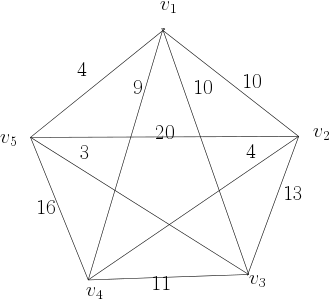
\includegraphics[width=0.5\textwidth]{2.17.png}
  \caption{}
\end{figure}
\noindent 根据分支与界法的算法流程,我们首先对10 条边进行排序:\\
\begin{align*}
  e_{3,5}&\quad e_{2,4} \quad e_{1,5} \quad e_{1,4} \quad e_{1,2} \quad e_{1,3}\quad e_{3,4}\quad e_{2,3}\quad  e_{4,5}\quad e_{2,5}\\
  3 &\qquad 4 \quad \quad 4 \qquad 9\quad 10\qquad 10\quad 11\qquad 13\qquad 16\qquad 20
\end{align*}
\indent 最初$d_0 = +\infty$。我们第一次选的5 条边为:$e_{3,5},e_{2,4},e_{1,5},e_{1,4},e_{1,2}$。\\
\indent 因为他们不构成H回路。接下来我们删去$e_{1,2}$,加入$e_{1,3}$,得到:$e_{3,5},e_{2,4},e_{1,5},e_{1,4},e_{1,3}$。\\
\indent 他们依然不构成H回路。接下来我们得到:$e_{3,5},e_{2,4},e_{1,5},e_{1,4},e_{3,4}$。\\
\indent 他们依然不构成H回路。接下来我们得到:$e_{3,5},e_{2,4},e_{1,5},e_{1,4},e_{2,3}$。\\
\indent 此时栈中5 条边构成H 回路,我们更新$d_0 = 33$。接下来我们删去$e_{1,4},e_{2,3}$,继续搜索得到:$e_{3,5},e_{2,4},e_{1,5},e_{1,2},e_{1,3}$。\\
\indent 此时栈中5 条边不构成H回路。接下来我们得到:$e_{3,5},e_{2,4},e_{1,5},e_{1,2},e_{3,4}$。\\
\indent 此时栈中5 条边构成H回路,我们更新$d_0 = 32$。接下来我们删去$e_{1,2},e_{3,4}$,继续搜索得到:$e_{3,5},e_{2,4},e_{1,5},e_{1,3}$\\
\indent 此时栈中存在回路,我们删去$e_{1,3}$,继续搜索得到:$e_{3,5},e_{2,4},e_{1,5},e_{3,4},e_{2,3}$ 此时栈中边的权值和为$35>d_0$,我们删去$e_{3,4},e_{2,3}$,继续搜索。\\
\indent 此后,栈中边要么构成回路,要么边权和> d0,直到算法结束都无法构成回路,所以最后求得的最优解为$32$。\\
\indent 从以上分析我们可以知道,分支与界法对于边权和大于等于当前界值和必定不合法的分支都不再搜索,而且最后得到的界值就是问题的最优解。从该例看,分支与界法比穷举搜索法要优秀得多,但是在最坏情况下,其计算复杂度仍然为阶乘级别的。因此在实际问题中,人们经常采用近似算法求得问题的近似最优解,从而避免浩瀚的计算量。\\
\end{sample}
\subsection{便宜算法}
\indent 在设计近似算法时,往往需要对原问题增加一些限制,以便能够提高计算速度和近似效果,而这些限制又常常都是比较符合实际的。在这里我们介绍\textbf{“便宜算法”(又称最近邻算法)},他需要问题满足下面两个限制:\\
\begin{enumerate}
  \item G 是无向正权图;
  \item G 的边权符合三角不等式,即任意三个点构成的三角形中较小的两边的权值和大于等于第三边的权值和。
\end{enumerate}
\indent 便宜算法基于的是一种贪心的思想,在最初时维护的是一个边权和为0 的自环,每次选取一个未在回路中且距离回路最近的点,贪心地将其加入回路,得到一个新回路。重复这个过程,直到得到H 回路。\\
下面是算法的伪代码:\\
\begin{algorithm}
\renewcommand{\algorithmicrequire}{\textbf{Input:}}
\renewcommand\algorithmicensure {\textbf{Output:}}
    \caption{便宜算法}
    \begin{algorithmic}[1]
      \label{alg:pysf}  %state命令是开始算法,这是会有默认的编号产生
      \STATE $T\leftarrow\{(1,1)\}$
      \WHILE{T不是H回路}
          \STATE $u\leftarrow$不在T中且距离T 最近的点
          \STATE $v\leftarrow$在T 中且距离u 最近的点
          \STATE $v_1, v_2 \leftarrow v$在T 中相邻的节点
          \IF{$w(u,v_1) − w(v,v_1)\leq w(u,v_2)−w(v,v_2)$}
             \STATE $ T\leftarrow T −\{(v_1,v)\} + \{(u,v),(u,v_1)\}$
          \ELSE{}
              \STATE  $ T\leftarrow T −\{(v_2,v)\} + \{(u,v),(u,v_2)\}$
          \ENDIF
      \ENDWHILE

    \end{algorithmic}
\end{algorithm}
\indent 其中将u 加入v 的前面或后面是根据回路T 的长度的增量贪心确定的,这也便是“便宜”的含义。
\begin{sample}\K
已知下面的权矩阵,其旅行商问题采用便宜算法近似求解的过程如图2.18所示。\\
\textbf{答案:}最后得到的最优解为109。
$$\left[
  \begin{array}{ccccc}
    0  & 18 & 35 & 25 & 27 \\
    18 & 0 & 23 & 21 & 19 \\
    35 & 23 & 0 & 17 & 28 \\
    25 & 21 & 17 & 0 & 24 \\
    27 & 19 & 28 & 24 & 0 \\
  \end{array}
\right]$$
\begin{figure}[H]
  \centering
  % Requires \usepackage{graphicx}
  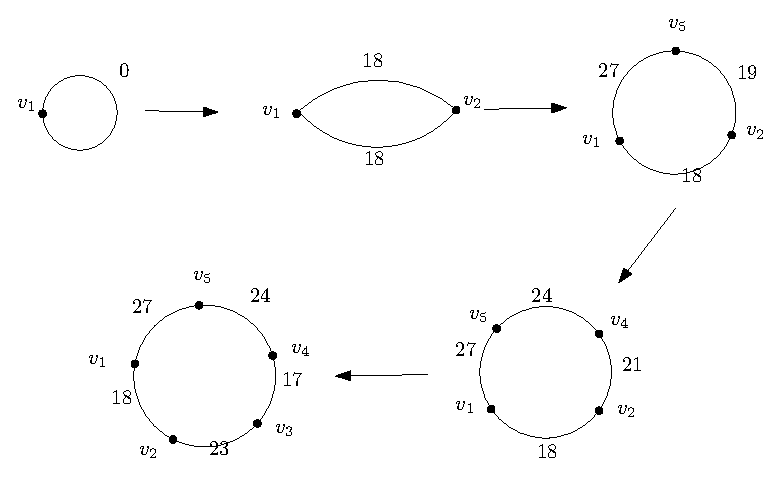
\includegraphics[width=0.9\textwidth]{2_19.eps}
  \caption{}
\end{figure}

\end{sample}
\begin{theorem}\H
设正权完全图的边权满足三角不等式,其旅行商问题的最佳解释$O_n$,便宜算法的最优
解是$T_n$,则$\frac{T_n}{O_n} < 2$。\\
\textbf{证明:}设往初级回路T 中每加入一个节点u后,T的权值和增量为$\delta_u$; $\delta_u=w_{uv} +w_{uv'} −w_{vv'}$,
我们将证明$\delta_u$与最佳解中的某条边(设其长度为$l_u$)形成对应,并且满足$\delta_u\leq2l_u$。\\
\indent 初始时T = {(1,1)},设$O_n$ 中与1相关联的边权较小的一条边为e,e的权值为$l_u$。\\
当加入一个点u后,由于u是离1 最近的点,故w(1,u) 当然不会大于$l_u$,自然有$\delta_u\leq2l_u$。在$O_n$中删去e 后,我们继续往T中加入点。\\
\begin{figure}[H]
  \centering
  % Requires \usepackage{graphicx}
  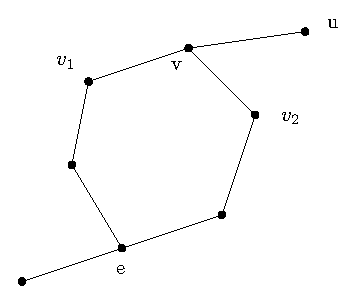
\includegraphics[width=0.8\textwidth]{2_20.eps}
  \caption{}
\end{figure}
\indent 此时,$O_n$中肯定会有一些尚未被删去的边与T中的点相关联,否则与$O_n$ 是H回路矛盾。\\
设其中一边权最小的一条为e,其边权为$l_u$。假定算法此时加的边为$(u,v)$。 则:
\begin{equation}
  w(u,v)\leq l_u
\end{equation}
由边权满足三角不等式知:\\
\begin{gather}
  w(u,v_i)\leq w(u,v) + w(v,v_i); \quad i = 1, 2\\
  w(u,v_i) \leq l_u + w(v,v_i); \quad i = 1,2
\end{gather}
由式2.1、式2.3得:
\begin{equation}
  \delta_u \leq 2l_u
\end{equation}
\indent 此时$\delta_u $与$O_n$ 中的边e对应,在$O_n$中删去e,并重复这个过程,可知每个$\delta_u$ 与最佳解
中的某条边形成对应,故$T_n < 2O_n$。
\paragraph{}便宜算法的计算复杂度是$O(n^2)$。其效率比枚举法或分支与界法要高得多。虽然从理论上说它的近似程度并非理想,但是在实际上它与最优解常常十分接近。如例2.7.2 的最优解是107,而便宜算法的解是109。
\end{theorem}
\subsection{最短路径}
\indent 在路上骑车穿梭的时候,我们常常会想要尽快地到达目的地,却不知道应该走哪条路。如果我们把路的交叉口看作是点,把路看作是边并以路的长度为权值,并且规定只能在交叉口转弯换路(毕竟跨越花坛并不是很文明的行为),那么整个学校就可以看做是一个无向图。而这些困扰我们的问题,就转化为了无向图上两个点之间的\textbf{最短路径问题}。\\
\paragraph{}由于很多情况下,路并不都是双向的,存在单行道的说法,使得原图成为了一个混合图,不利于我们形式化地去分析问题。所以,对原图进行一个简单的转化:\\
去掉所有的无向边${v_i,v_j}$ 并相应地添上两条有向边$(v_i,v_j)$ 与$(v_j,v_i)$, 边权$w(v_i,v_j) = w(v_j,v_i) = w{v_i,vj}$。
原图就转化为了一个等价的有向图。记从$v_s$出发到$v_i$的最短路的长度为$\pi(v_s,v_i)$,简记$\pi(v_s, v_i)$ 为$\pi(v_i)$。
\paragraph{三类模型}\K {最短路径问题按照实际问题的模型,包括三类模型:}\\
\begin{enumerate}
  \item 某两结点之间的最短路径
  \item 某结点到其他各结点的最短路径
  \item 任意两结点之间的最短路径
\end{enumerate}
容易分析,模型(2)如果能够解决,模型(1)和(3)自然可以解决。
\paragraph{最短路径}相关概念及前提:\\
\begin{itemize}
  \item[-] 不失一般性,我们研究$v_1$到其他各结点的最短路径
  \item[-] $v_1$到$v_i$的一条路径的长度记为$\pi_{(i)}$,且$$\pi_{(i)}=\sum_{e\in P(i)}w(e)$$\\
  其中,$w(e)$表示$e=(v_j,v_k)$的权,也记为$w_{jk}$
  \item[-] $v_1$到$v_i$的最短路径就是$\pi(i)$的最小值
\end{itemize}
\subsection{最短路径-正权图}
\begin{lemma}\K
正权图$G$中,如果是$v_1$到$v_i$的一条最短路,且$v_j\in P(i)$,则$P(j)$是$v_1$到$v_j$的一条最短路。\\
\textbf{证明:}
\begin{figure}[H]
  \centering
  % Requires \usepackage{graphicx}
  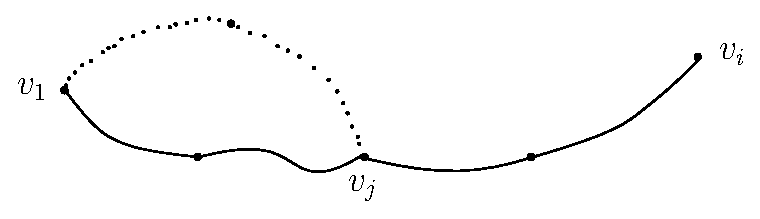
\includegraphics[width=0.8\textwidth]{2_6_1.eps}\\
  \caption*{}
\end{figure}
\end{lemma}
\begin{lemma}\K
正权图中任意一条最短路径的长度大于其局部路径长度。\\
\textbf{证明:}结论显然
\end{lemma}
\subsection{Dijkstra(迪克斯特拉)算法}
\textbf{算法过程描述:}\\
\begin{enumerate}
  \item 每个结点用从源结点沿已知最佳路径到本结点的距离来\textcolor[rgb]{1.00,0.00,0.00}{标注},标注分为\textcolor[rgb]{1.00,0.00,0.00}{临时性标注}和\textcolor[rgb]{1.00,0.00,0.00}{永久性标注},最新永久标注节点为\textcolor[rgb]{1.00,0.00,0.00}{工作节点}。
  \item 初始时,所有结点都为临时性标注,标注为无穷大;
  \item 将源结点标注为$0$,且为永久性标注,并令其为工作结点;
  \item 检查与工作结点相邻的临时性结点,若该结点到工作结点的距离与工作结点的标注之和小于该结点的临时标注,则用新计算得到的和重新标注该结点
  \item 在整个图中查找具有最小值的临时性标注结点,将其变为永久性结点,并成为下一轮检查的工作结点;
  \item 重复第四、五步,直到目的结点成为工作结点。
\end{enumerate}
\paragraph{Dijkstra算法应用举}找出从A到D的最短路径\\
$1)$每个结点用从源结点沿已知最佳路径到本结点的距离来标注,标注分为临时性标注和永久性标注
\begin{figure}[H]
  \centering
  % Requires \usepackage{graphicx}
  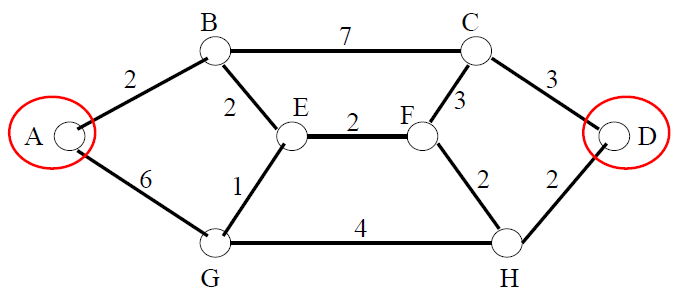
\includegraphics[width=0.8\textwidth]{dj1.png}\\
  \caption*{}
\end{figure}
$2)$初始时,所有结点都为临时性标注,标注为无穷大;
\begin{figure}[H]
  \centering
  % Requires \usepackage{graphicx}
  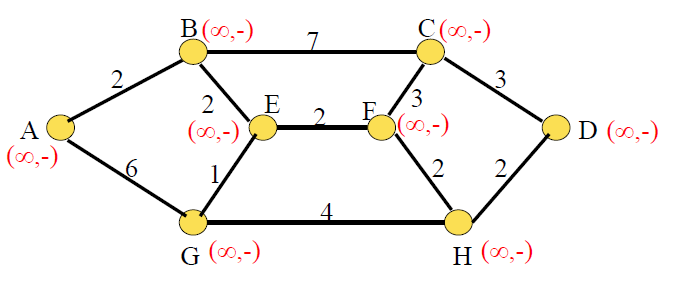
\includegraphics[width=0.8\textwidth]{dj2.png}\\
  \caption*{}
\end{figure}
3)将源结点标注为$0$,且为永久性标注,并令其为工作结点;
\begin{figure}[H]
  \centering
  % Requires \usepackage{graphicx}
  \includegraphics[width=0.8\textwidth]{dj3.png}\\
  \caption*{}
\end{figure}
4)检查与工作结点相邻的临时性结点,若该结点到工作结点的距离与工作结点的标注之和小于该结点的临时标注,则用新计算得到的和重新标注该结点
\begin{figure}[H]
  \centering
  % Requires \usepackage{graphicx}
  \includegraphics[width=0.8\textwidth]{dj4.png}\\
  \caption*{}
\end{figure}
5)在整个图中查找具有最小值的临时性标注结点,将其变为永久性结点,并成为下一轮检查的工作结点;
\begin{figure}[H]
  \centering
  % Requires \usepackage{graphicx}
  \includegraphics[width=0.8\textwidth]{dj5.png}\\
  \caption*{}
\end{figure}
6)重复第四、五步,直到目的结点成为工作结点。
\begin{figure}[H]
  \centering
  % Requires \usepackage{graphicx}
  \includegraphics[width=0.8\textwidth]{dj6.png}\\
  \caption*{}
\end{figure}
最终结果:
\begin{figure}[H]
  \centering
  % Requires \usepackage{graphicx}
  \includegraphics[width=0.8\textwidth]{dj8.png}\\
  \caption*{}
\end{figure}
\begin{figure}[H]
  \centering
  % Requires \usepackage{graphicx}
  \includegraphics[width=0.8\textwidth]{dj9.png}\\
  \caption*{}
\end{figure}
Dijkstra算法的计算复杂度为O(n2)\\
\subsection{边权为1 时v1 到各点的最短路}
\indent 边权值均为1 的图,Dijkstra 算法就等价于广探法。因而我们可以直接用广探法求得最短路径。\\
\paragraph{算法流程}使用队列Q模拟广探法
\begin{shaded}
\textbf{算法:广探法}
\begin{enumerate}
  \item 置\begin{equation*}
    S=\emptyset ,Q={v_1} ,\pi(i)=
   \begin{cases}
   0 &\mbox{i=1}\\
    \infty &\mbox{$i\neq 1$}
   \end{cases}
  \end{equation*}
  \item 取出队头元素,记此元素为$v_j$,并弹出队头。置$S\leftarrow S +{v_j}$。若$S = V$ ,算法结束,否则转3。
  \item 对所有$v_i\in V-S\bigwedge(v_j,v_i)\in E$,$\pi(i)=\pi(j)+1$,并将$v_j$加入队尾。转2
\end{enumerate}
\end{shaded}
\indent 同样,为了求出路径,我们可以加入一个$n$ 维向量$prev$,初始所有分量皆为$-1$。对步骤3稍加修改:\\
\indent $v_i\in V-S\bigwedge(v_j,v_i)\in E$,\\
\indent $\pi(i)=\pi(j)+1$,\\
\indent $prev(i)\leftarrow j$
\begin{sample}\K
使用广探法求图2.20 中$v_1$到其余各点的最短路径过程如下:\\
\begin{figure}[H]
  \centering
  % Requires \usepackage{graphicx}
  \includegraphics[width=0.7\textwidth]{2.201.png}\\
  \caption{}
\end{figure}
\begin{align*}
  1. &S=\emptyset,Q=\{v_1\},\pi=\{0,\infty,\infty,\infty \},prev=\{-1,-1,-1,-1\} \\
  2. &j=1,S=\{v_1\},Q=\{v_2,v_3\},\pi=\{0,1,1,\infty\},prev=\{-1,1,1,-1\}\\
  3. &j=2,S=\{v_1,v_2\},Q=\{v_3,v_4\},\pi=\{0,1,1,2\},prev=\{-1,1,1,2\}\\
  4. &j=3,S=\{v_1,v_2,v_3\},Q=\{v_4\},\pi=\{0,1,1,2\},prev=\{-1,1,1,2\}\\
  5. &j=4,S=\{v_1,v_2,v_3,v_4\}\\
\end{align*}
\end{sample}
\begin{theorem}\H
如果图$G$是以正向表或邻接表的数据结构表示,则本算法的计算复杂性为$O(m)$\\
\end{theorem}
\subsection{Ford算法}
存在负边权时,Dijkstra 算法的正确性便得不到保证,如图2.21
\begin{figure}[H]
  \centering
  % Requires \usepackage{graphicx}
  \includegraphics[width=0.5\textwidth]{2.211.png}\\
  \caption{}
\end{figure}
$v_1$ 到$v_2$ 的最短路长应为8,但是通过Dijkstra 算法得到的结果为9。\\
为了解决这一问题,Ford 给出了新的算法:\\
\begin{figure}[H]
  \centering
  % Requires \usepackage{graphicx}
  \includegraphics[width=0.3\textwidth]{ford.eps}\\
  \caption*{}
\end{figure}
\begin{enumerate}
  \item 置$\pi(1)=0,\pi(i)=\infty,$
  \item i从2到n,令$$
  \pi\leftarrow min [\pi(i),min(\mathop{\pi(j)}\limits_{j\in\Gamma_i^-} + w_{ji}) ]
  $$
  \item 若全部$\pi(i)$都没变化,结束。否则转(2)
\end{enumerate}
\textbf{证明:}
设算法结束时,对某个结点$v_s$有$\pi(s)$。\\
设$v_1$到$v_s$之间存在某条路径如下:$$\mu=(1,t_h,t_{h-1},\cdots,t_1,s)$$
根据算法步骤(2),我们可以得到如下等式:\\
$$\pi(s)=min(\pi(s),min((\pi(t_1)+w(t_1,s)),\cdots ))$$
显然,我们可以得到不等式:\\
\begin{gather*}
               \pi(s)  \leq \pi(t_1)+w(t_1,s) \\
               \pi(s)  -\pi(t_1)\leq w(t_1,s)\\
               \pi(t_1)  -\pi(t_2)\leq w(t_2,t_1)\\
               \cdots\\
               \pi(t_h)  -\pi(1)\leq w(1,t_h)
\end{gather*}
即:$$\pi(s)\leq w(t_1,s)+w(t_2,t_1)+\cdots+w(1,t_h)$$

如果果G中负权边很少,可以先删掉它们,采用Dijkstra算法计算,然后再开始迭代过程,可提高计算效率。\\
\textbf{思考}在正权图中采用FORD算法,同Dijkstra算法会有什么区别?\\
\begin{theorem}\H
在最坏情况下Ford 算法的计算复杂性是O(mn)。
\end{theorem}
\begin{sample}\K
使用Ford 算法求图2.22中$v_1$到其他各结点的最短路径的过程如下:\\
\begin{figure}[H]
  \centering
  % Requires \usepackage{graphicx}
  \includegraphics[width=0.6\textwidth]{2_22.eps}\\
  \caption{}
\end{figure}
\begin{flushleft}
  \begin{align*}
  1. &  \pi=(0,\infty,\infty,\infty)\\
  2. &  \pi=(0,1,2,2)\\
  3. & \pi=(0,-2,2,-1)\\
  4. & \pi=(0,-2,2,1)
\end{align*}
\end{flushleft}
\end{sample}
\section{关键路径}
\paragraph{}现实中有很多工程问题,建水坝、造飞机、组装机床、软件开发...,都会包含很多工序。\\
工序与工序之间很多都存在先后次序关系,一般这些次序关系是预知的。\\
对于工程领导人员来说:\\
\begin{description}
  \item[-] 了解工程最少需要多少时间
  \item[-] 要害工序是哪些
\end{description}
此类问题,如何转化为图论问题解决?\\
\subsection{PT图}
\textbf{PT(Potentialask graph)图:}\\
\begin{itemize}
  \item[-] 用结点表示工序
  \item[-] 用有向边表示工序间的次序关系
  \item[-] 用边权值表示工序所需要的时间
\end{itemize}
\begin{figure}[H]
  \centering
  % Requires \usepackage{graphicx}
  \includegraphics[width=0.6\textwidth]{pt.png}\\
  \caption*{}
\end{figure}
\textbf{PT图的特点}\\
\begin{itemize}
  \item[.] 从某结点出发的边,权值均相等
  \item[.] 必定不存在有向回路
  \item[.] 存在没有入度和没有出度的结点
\end{itemize}
\begin{sample}\K
一项工程任务,大到建造一座水坝,一枚航天火箭,一座体育中心,小至组装一台机床,一家电视机,都要包括许多工序。这些工
序相互约束,只有在某些工序完成之后,一个工序才能开始。即它们之间存在完成的先后次序关系,一般认为这些关系是预知的,而且也能够预计完成每个工序所需要的时间。这时工程领导人员迫切希望了解最少需要多少时间才能够完成整个工程项目,影响工程进度的要害工序是哪几个?\\
\begin{table}[!ht]
  \centering
  \begin{tabular}{|c|c|c|c|}
\hline
  序号 &  名称 &  所需时间 & 先后工序  \\
\hline
 1 &  基础设施  &  15 &  \\
\hline
 2 & 下部砌砖 &  5 &  1 \\
\hline
 3 & 电线安装 &  4 &  1\\
\hline
 4 &   圈梁支模&   3&  2\\
\hline
 5 &  水暖管道 &   4&  2\\
\hline
6 &  大梁安装 &  2 &  4,5 \\
\hline
 7 &   楼板吊装&   2&  6,9,10\\
\hline
 8 &  楼板浇模 &  3 &  6,9,10\\
\hline
 9 &  吊装楼梯 & 3 &  4,5\\
\hline
 10 &  上部砌砖 &   4&  2 \\
\hline
\end{tabular}
  \caption{}
\end{table}
相应的PT图如图2.23所示,图中$v_i$ 表示作业$i$,以$v_i$ 为始点的边权是作业$v_i$ 的时间。作业$v_i$最早开始时间应在以$v_i$为终点的作业完成之后。\\
整个工程最短完成时间应该是:从$v_1$到$v_11$的最长路径,该路径也是工程的关键路径。
\begin{figure}[H]
  \centering
  % Requires \usepackage{graphicx}
  \includegraphics[width=0.6\textwidth]{2_23.eps}\\
  \caption{}
\end{figure}
\end{sample}

\begin{lemma}\H
不存在有向回路的图G中,一定存在负度及正度为零的结点。\\
\textbf{证明(构造法):}\\
\begin{itemize}
  \item[-] 在$G$中构造一条极长的有向道路$P$,并设$P$的起点为$v_i$,终点为$v_j$,则一定有$d^{-}(v_i)=0,d^{+}(v_j)=0$
  \item[-] 否则,假定$d^{-}(v_i)\neq 0$,则一定有边$(v_k,v_i)\in E(G)$\\
  若 $v_k\in P$,则$G$存在有向回路;\\
  若 $v_k \notin P$,则P不是极长道路。因此$d^{-}(v_i)=0$
  \item[-] 同理,可证$d^{+}(v_j)=0$
\end{itemize}
\end{lemma}
\begin{lemma}
设G不存在有向回路,可以将G的结点重新编号为$v_1',v_2',\cdots,v_n'$,使得对任意的边$(v_i',v_j')\in E(G)$,都有$i<j$\\
\textbf{证明:}\\
\begin{itemize}
  \item[-] 根据引理2.8.1,G中存在$v_i$,满足$d^{-}(v_i)=0$对之重新编号$v_1'$
  \item[-] 在G中删掉$v_i$ ,得到$G'=G-v_1'$,可知,G’为G的导出子图,因此没有有向回路,因此必然存在负度为零的结点
  \item[-] 将G'中负度为零的结点编号为$v_2'$,再做$G'-v_2'$
  \item[-] 依次类推,可以将G的全部结点重新编号。
  \item[-] 此时,G中所有边的编号均为从编号小的结点指向编号大的结点,否则与编号原则相悖
\end{itemize}
\end{lemma}
\begin{shaded}
PT图中最长路径算法:\\
\\
-(1) 对结点重新编号$v_1',v_2',\cdots,v_n'$\\
-(2) $\pi(v_1')\leftarrow 0$\\
-(3) 对于j从2到n,令$$\pi(v_j')=\mathop{max}\limits_{v_i'\in \Gamma^{-}(v_j')}(\pi(v_i')+w(v_i',v_j'))$$\\
-(4)End!\\
该算法计算复杂性为O(m)\\
\end{shaded}
\indent 上述算法将得到最长路径就是工程的关键路径。\textcolor[rgb]{1.00,0.00,0.00}{路径长度即为工程的最早完成时间}。\\
\textbf{思考:}\\
对于非关键路径上的工序,是否可以延误,如果可以,最多可延误多长时间?\\
\begin{sample}
在例子2.8.1 中设$\pi(v_n)$是工程完工的最早时间,设工序$i$到工程完工最少需要的时间为$\pi(v_i,v_n)$,则工序$i$的最晚启动时间应该是\\
\begin{equation}
    \tau(v_i)=\pi(v_n)-\pi(v_i,v_n)
\end{equation}
其中$\pi(v_i,v_n)$表示$v_i$到$v_n$的最长路长度。\\
 这样每个节点$v_i$有两个值:\\
(1)最早启动时间$\pi(v_i)$\\
(2)最晚启动时间$\tau(v_i)$\\
 允许延误的时间为:$t(v_i)=\pi(v_i)-\tau(v_i)$\\
则重新计算例子2.8.1中各点的$\pi(v_i),\tau(v_i)$\\
\begin{table}[H]
  \centering
\begin{tabular}{|c|c|c|c|c|c|c|c|c|c|c|c|}
  \hline
  % after \\: \hline or \cline{col1-col2} \cline{col3-col4} ...
   结点& 1& 2 & 3 &4 & 5 & 6 & 7& 8 & 9 & 10 & 11 \\
   \hline
  $\pi(v_i)$ & 0 & 15 & 15 & 20 & 20 & 24 & 24 & 20 & 27 & 27 & 30 \\
  \hline
  $\tau(v_i)$ & 0 & 15 & 26 & 21 & 20 & 25 & 24 & 23 & 28 & 27 & 20 \\
  \hline
\end{tabular}
\end{table}
从上面可以看出,最长路径即关键路径上各工序是不允许延误的,否则会延误整个工程进度。\\
\end{sample}
\subsection{PERT(Programme evaluation and review technique)图}
\indent PERT图采用有向边表示工序,权值表示工序所需要的时间,关键路径算法与PT图相同,工序最晚启动时间算法略有不同。\\
\indent 在PERT图中,采用有向边表示工序,其权值表示该工序所需时间。如果工序$e_i$完成后$e_j$ 才能开始,则令$v_k$ 是$e_i$ 的终点,$e_j$ 的始点。\\
根据这种约定,例2.8.1 的PERT 图如图2.24,其中$\mathop{i}\limits_{-} $表示工序i。
\begin{figure}[H]
  \centering
  % Requires \usepackage{graphicx}
  \includegraphics[width=0.6\textwidth]{2_24.eps}\\
  \caption{}
\end{figure}
 同样,PERT 图中不存在有向回路。而且与PT 图类似,PERT 图中工程的最早完工时间是$v_1$ 到$v_n$ 的最长路径长度,这条路径就是\textbf{关键路径}。\\
工序$e_k=(v_i,v_j)$的最早启动时间是$\pi(v_i)$,最晚启动时间是$\tau(v_i,v_j)=\pi(v_n)-\pi(v_i,v_n)-w(v_i,v_j)$。其中$\pi(v_i,v_n)$是$v_i$到$v_n$的最长路径,$w(v_i,v_j)$是该工序所需的时间。\\
这样工序$e_k=(v_i,v_j)$的允许延误的时间$t(v_i,v_j)=\tau(v_i,v_j)-\pi(v_i)$。\\
\indent 由最长路径算法可以求出$\pi(v_i')$,为了便于计算$\tau(v_i',v_j')$,可先作简单变换。由于$$\tau(v_j')=\pi(v_n')-\pi(v_j',v_n')$$
故$$\tau(v_i',v_j')=\tau(v_j')-w(v_i',v_j')$$
即得$$\tau(v_i',v_j')=\tau(v_j')-\pi(v_i')-w(v_i',v_j')$$
这样可以使用PT图中最长路径算法求$\tau(v_j')$。\\
以图2.24为例,其计算结果是(设已回到原结点号):
\begin{align}
             &\pi(1)=0,\pi(2)=15,\pi(3)=20,\pi(4)=27,\pi(5)=24,\pi(6)=30        \\
             &\tau(1)=0, \tau(2)=15,\tau(3)=20,\tau(4)=27,\tau(5)=24,\tau(6)=30\\
             &\tau(\mathop{1}\limits_{-})=0,\tau(\mathop{2}\limits_{-})=0,\tau(\mathop{3}\limits_{-})=11,\tau(\mathop{4}\limits_{-})=1,\tau(\mathop{5}\limits_{-})=0,\tau(\mathop{6}\limits_{-})=1\\
              &  \tau(\mathop{7}\limits_{-})=1,\tau(\mathop{8}\limits_{-})=0,\tau(\mathop{9}\limits_{-})=0,\tau(\mathop{10}\limits_{-})=3
\end{align}
\indent 与PT图一样,PERT图的计算复杂度也是O(m)。\\
\chapter{树}
\section{树的有关定义}
\subsection{基本定义}
\begin{defination}
树的基本定义\begin{description}
        \item[树] :一个不含任何回路的连通图, 用T 表示
        \item[树枝]: T中的边,称为T 的树枝
        \item[树叶] :T 中度为一的结点
      \end{description}
\end{defination}
\begin{defination}
设e是G的一条边,若$G'=G-e$比G的连通支数增加,则称e是G的一条割边。\\
\begin{figure}[H]
  \centering
  % Requires \usepackage{graphicx}
  \includegraphics[width=0.7\textwidth]{3_1.eps}\\
  \caption{}
\end{figure}
\end{defination}
\begin{theorem}
$e=(u,v)$是割边,当且仅当e不属于G的任何回路。\\
\textbf{证明:}\\
\begin{itemize}
  \item 充分性(反证法):若$e=(u,v)$属于G的某个回路,则$G'=G-e$中仍存在u到v的道路,故结点u和v属于同一连通支,e不是割边。
  \item 必要性(反证法):反之,若e不是割边,则$G'$和G
的连通支数一样,因此u和v仍然处在同一个连
通支,因此在图$G'$中存在道路$P(u,v)$ $$P(u,v)+e$$就是图G的一个回路.
\end{itemize}
\end{theorem}
\begin{theorem}
$e=(u,v)$是割边,当且仅当e不属于G的任何回路。\\
\end{theorem}
\textbf{小结论:}
\begin{itemize}
  \item \textcolor{red}{树的每条边都不属于任何回路}
  \item \textcolor{red}{因此树的每条边都是割边}
  \item \textcolor{red}{树是边数最少的连通图}
\end{itemize}
\subsection{树的等价性质}
\begin{theorem}
设T 是结点数为$n\geq2 $的树, 则下列性质等价:
\begin{enumerate}
  \item T连通且无回路
  \item T 连通且每条边都是割边
  \item T连通且有n-1 条边
  \item T 有n-1 条边且无回路
  \item T的任意两结点间有唯一道路
  \item T 无回路,但在任意两结点间加上一条边后恰有一个回路
\end{enumerate}
{\hwxw 依次证明上述定理的正确性:}
{\song
\begin{itemize}
  \item (1)T连通且无回路$\Rightarrow$(2)T连通且每条边都是割边\\
  \textbf{证明:}\\
  由定理$3.1.2$ ,$e=(u,v)$是割边$\Leftrightarrow$ e 不属于G的任何回路.
  \item (2)T 连通且每条边都是割边$\Rightarrow$ (3)T 连通且有n-1 条边\\
  \textbf{证明:}\\
  采用数学归纳法: 对结点数n 进行归纳。\\
  设m(T) 为树T 的边数,n(T) 为树T 的结点数。\\
  n=2 时, 结论显然成立;\\
  设$n\leq k$ 时,$m(T)=n(T)-1$ 成立。\\
  当n=k+1 时, 由于每条边都是割边, 因此图$G'=G - e$ 有两个连通支$T_1$和$T_2$。\\
  根据假设,$$ m(T_1)=n(T_1)-1,\quad m(T_2)=n(T_2)-1 \Rightarrow m(T)=m(T_1)=m(T_2)+1=n(T)-1$$
  \item (3)T 连通且有n-1条边$\Rightarrow$(4)T 有n-1 条边且无回路 \\
  \textbf{证明:}\\
  反证法: 假定T 有回路。\\
    设C 为其中一条含有k 个结点的初级回路,故回路内有k 条边。考察C 以外的$n-k $个结点, 为保持T 的连通性, 至少需要C 以外的n-k 条
    边。所以T 的边数至少为$k+(n-k)=n$ 条与T 有$n-1$ 条边矛盾,故假设不成立,即T 无回路。
  \item(4) T有$n-1$ 条边且无回路$\Rightarrow$ (5)T 的任意两结点间有唯一道路\\
  \textbf{证明:}\\
  首先证明任意两结点间道路的存在性(反证法) : 设$u,v$ 是T 的任
意两结点, 假设不存在道路$P(u,v)$ 则$u,v$ 属于两个连通支$T_1,T_2$。 由于$m=n-1$, 则至少有一个连通支的边数不少于结点数。不妨
设为$T_1,m(T_1)\geq n(T_1)$ 设$T_1$ 无回路,由性质(1)$\Rightarrow$ 性质(2)
$\Rightarrow$性质(3),$m(T_1)=n(T_1)-1<n(T_1)$,矛盾。因此此时该连通支
$T_1$ 必存在回路, 与题目前提矛盾! 因此, $P(u,v)$ 存在。\\
其次证明任意两结点间道路的唯一性:\\
如图$3.2$, 若存在两条不同的道路$P(u,v), P'(u,v)$,则$P(u, v)\bigoplus P'(u, v)$
必存在回路。与题目假设矛盾。因此$P(u,v)$ 唯一。
\begin{figure}[H]
  \centering
  % Requires \usepackage{graphicx}
  \includegraphics[width=0.6\textwidth]{3.2.png}\\
  \caption{}
\end{figure}
\item (5)T的任意两结点间有唯一道路$\Rightarrow \quad $ (6)T 无回路, 但在任意两结点间
加上一条边后恰有一个回路\\
\textbf{证明:}\\
 首先证明T 无回路:\\
若T 有回路,则回路上任意两点之间至少有两条不同的道路,与
前提矛盾。\\
故T 无回路。\\
 其次证明在任意两结点间加上一条边e 后恰有一个回路:\\
设原来两结点之间的道路为P,则$P\bigcup e $即为一个回路。\\
故在任意两结点间加上一条边e 后恰有一个回路\\

\item (6)T 无回路, 但在任意两结点间加上一条边后恰有一个回路$\Rightarrow \quad$ (1)T
连通且无回路\\
\textbf{证明:}
 T 连通:因任意两结点间加上一条边后恰有一个回路,故原图中
任意两点间必然存在一条道路。\\
T 无回路:已知条件
\end{itemize}
}
\end{theorem}
\begin{theorem}
树T中一定存在树叶结点\\
{\song
\textbf{证明:}\\
T为连通图,故不存在度为零的结点。\\
假设T中不存在树叶结点,则意味着不存在度为
1的结点,则所有结点度均不小于2。
$$ m=\frac{1}{2}\sum_{v\in V(G)} d(v)\quad \Rightarrow \quad m \geq \frac{1}{2}\cdot 2n=n > n-1$$
容易看出:矛盾!\\
}
\end{theorem}
\begin{defination}
如果T是图G的支撑子图,而且又是一棵树,则称T是G的一棵\textcolor{red}{支撑树},或称\textcolor{red}{生成树},又简称为G的\textcolor{red}{树}。
\end{defination}
\subsection{余树的概念}
\begin{defination}
G中删掉T的各边后子图称为T的\textcolor{red}{余树},记为$\bar{T}$
\end{defination}

\section{基本关联矩阵及其性质}
{\hwxw 本节研究的范围是有向连通图。}\\
\begin{defination}
有向连通图$G = (V , E)$ 的关联矩阵$B $中划去任意节点$v_k$ 所
对应的行,得到一个$(n−1)\times m$ 的矩阵$B_k$, $B_k$ 称为G 的一个基本关联矩阵。
\begin{figure}[H]
  \centering
  % Requires \usepackage{graphicx}
  \includegraphics[width=0.6\textwidth]{3_3.eps}\\
  \caption{}
\end{figure}
\begin{equation}
B=\bordermatrix{%
       & e_1       & e_2     &e_3    &e_4  &e_5 &e_6\cr
v_1    & 1         & -1       &1     & 0 & 0 & 1\cr
v_2    & 0        & 0       &-1     & -1 & 0 & -1\cr
v_3    & -1         & 1       &0     &0 &1 &0
},
\end{equation}
\end{defination}
{\hwxw 下面我们来研究基本关联矩阵的性质。\\}
\begin{theorem}
有向图$G = (V , E)$ 关联矩阵B 的秩$ran(B) < n$。\\
{\song
\textbf{证明:}\\
关联矩阵特点:每一列都只有一个$1$和$-1$\\
n行全部相加\\
即n 个行向量线性相关,因此
$$ran B< n$$
证毕!
}
\end{theorem}
\begin{theorem}
设$B_0$是有向图G关联矩阵B的任意一k阶子方阵,则$det(B_0)$为$0,1$或$-1$\\
{\song
\textbf{证明:}\\
若$B_0$某列全零,则$det(B_0)=0$\\
若$B_0$每列都有两个非零元,则$det(B_0)=0$\\
若$B_0$存在某列只有一个非零元,则按该列展开可知$det(B_0)=\pm det(B_1)$\\
依次类推,可证!
}
\end{theorem}

\begin{theorem}
设$B_0$是有向图G关联矩阵B的任意一k阶子方阵,则$det(B_0)$为$0,1$或$-1$\\
{\song
\textbf{证明:}\\
若$B_0$某列全零,则$det(B_0)=0$\\
若$B_0$每列都有两个非零元,则$det(B_0)=0$\\
若$B_0$存在某列只有一个非零元,则按该列展开可知$det(B_0)=\pm det(B_1)$\\
依次类推,可证!
}
\end{theorem}

\begin{theorem}
设B是有向连通图G的关联矩阵,则$$ran B=n-1$$
{\song
\textbf{证明:}\\
设B中最少的线性相关行数为$l$\\
则$l\leq n$,其对应图中结点$v(i_1),v(i_2),\dots,v(i_l )$\\
\begin{equation*}
k_1\cdot b(i_1) +k_2\cdot b(i_2) +\cdots +k_l\cdot b(i_l) =O_m \quad (k_j\neq 0,\quad j=1,2,\cdots,l)
\end{equation*}
\begin{itemize}
  \item
  \begin{center}
    所有$b(i_j)$中,第$t(t=1,2,\cdots m)$个分量可能
  \end{center}
  \item
  \begin{center}
    所有$b(i_j)$中,第$t(t=1,2,\cdots m)$个分量可能
  \end{center}
  \item
  \begin{center}
    所有$b(i_j)$中,第$t(t=1,2,\cdots m)$个分量不可能
  \end{center}
\end{itemize}
  \begin{flushleft}
    否则,该分量最终不可能为$0$。
\end{flushleft}
\quad 这样,我们可以对矩阵B进行行、列交换,使前$l$行为线性相关的各行\\
\quad 再针对这$l$ 行中,有两个非零元的列换到前$r$列\\
则此$l$ 行中,其余$(m-r)$列将均为零元\\
\quad 此时矩阵B将变为
\begin{align*}
 B'= \begin{array}{lc}
\mbox{}&
\begin{array}{cc}r&m-r \end{array}\\
\begin{array}{c}l\\n-l\end{array}&
\left[\begin{array}{cc}
P&0\\
0&Q
\end{array}\right]
\end{array}
\quad \quad ran B=ran B'
\end{align*}
\quad 若$l <n$,则从$B'$可清楚看出,图G为两个连通支,这与
图G为连通图矛盾!\\
因此,一定有$l=n$
}
\end{theorem}
\begin{theorem}
设B是有向连通图G的关联矩阵,则$$ran B=n-1$$
\end{theorem}
\begin{theorem}
连通图G基本关联矩阵$B_k$的秩$$ran B_k=n-1$$
\end{theorem}
\begin{theorem}
设$B_k$为有向连通图G的基本关联矩阵,C为G中的一个回路。则C中各边所对应$B_k$的各列线性相关。\\
{\song
\textbf{证明:}\\
只需针对C为初级回路进行讨论即可\\
设C中含$l$个结点与$l$条边$(l<n)$,这$l$条边对应关联矩阵$B$中的$l$列,它们构成子阵$B(G_C)$  \\
\begin{figure}[H]
  \centering
  % Requires \usepackage{graphicx}
  \includegraphics[width=0.7\textwidth]{3.4.png}\\
  \caption{}
\end{figure}
\noindent C的关联矩阵为$l$ 阶方阵$B(C)$,据定理$3.2.5$ $$ran B(C)=l-1$$
说明$B(C)$的$l$列线性相关\\
观察$B(C)$与$B(G_C)$的关系:
{\hwxw
\begin{itemize}
  \item B(C)为$B(G_C)$的子阵,列数相同,行数不同
  \item C中各边只经过B(C)中的各结点,因此$B(G_C)$中其他结点对应各
行均为零
\end{itemize}
}
因此, $B(G_C)$的各列也线性相关!\\
因此,在$B_k$中,C对应各列也线性相关!\\
}
\end{theorem}
\begin{theorem}
设$B_k$为有向连通图G的基本关联矩阵,C为G中的一个回路。则C中各边所对应$B_k$的各列线性相关。\\
\end{theorem}
\begin{coro}
设H为连通图G的子图,如果H含有回路,
则H的\textcolor{red}{诸边}对应的G的基本关联矩阵各列线性相关。
\begin{figure}[H]
  \centering
  % Requires \usepackage{graphicx}
  \includegraphics[width=0.4\textwidth]{rank.png}\\
  \caption*{}
\end{figure}
\end{coro}
{\hwxw
思考:\\
有向连通图的基本关联矩阵,哪些列线性相关?\\
有向连通图的基本关联矩阵,哪些列线性不相关?\\
}
\begin{theorem}
令$B_k$是有向连通图G的基本关联矩阵,那么$B_k$的任意$n-1$阶子阵行列式非零的充要条件是其各列所对应的边构成G的一棵支撑树。
{\song
证明:\\
充分性:\\
设T为G的支撑树\\
子图T的基本关联矩阵$B_k(T)$是$n-1$阶子方阵,它的秩为$n-1$这意味着其行列式非零。\\
该子方阵恰好就是$B_k$的某个$n-1$阶子阵\\
即$B_k$所对应的该$n-1$阶行列式非零。\\
}
\end{theorem}
\begin{shaded}
{\hwxw
小结:\\
(1)有向连通图关联矩阵的秩\\
(2)有向连通图基本关联矩阵各列的线性相关性\\
(3)有向连通图基本关联矩阵同支撑树的关系\\
}
\end{shaded}

\section{支撑树的计数}
给定连通图G,其支撑树可以有多少个?\\
以某结点为根的支撑树可以有多少个?
\begin{figure}[H]
  \centering
  % Requires \usepackage{graphicx}
  \includegraphics[width=0.5\textwidth]{3_5.eps}\\
  \caption*{}
\end{figure}
\begin{theorem}
(Binet-Cauchy定理)已知两个矩阵$A=(a_{ij})_{m\times n}$
和$B=(b_{ij})_{n\times m}$,满足$m\leq n$,则$$ det(AB)=\sum_{i}(A_iB_i)$$
{\hwxw
其中$A_i$,$B_i$都是m阶行列式\\
$A_i$是从A中取不同的m列所成的行列式;\\
$B_i$是从B中取相应的m行构成的行列式;\\
结果为全部组合求和\\
}
\end{theorem}
\begin{sample}
已知$A=\left[
       \begin{array}{ccc}
         4 & 3 & 2 \\
         -2 & 4 & 3 \\
       \end{array}
     \right]
$\quad $B=\left[
           \begin{array}{cc}
             5 & 1 \\
             0 & 3 \\
             4 & 2 \\
           \end{array}
         \right]
$求$det(AB)$\\
解:\\
$AB=\left[
      \begin{array}{cc}
        28 & 17 \\
        2 & 16 \\
      \end{array}
    \right]
$\\
因此$det(AB)=28 \times 16-17\times 2=414$\\
\end{sample}
\begin{shaded}
\noindent 采用内比-柯西定理计算矩阵乘积的行列式通常比较复杂\\
其价值在于:揭示了乘积矩阵的行列式与各矩阵的子阵行列式之间的关系\\
连通图中不同支撑树的计数恰好利用了这种关系,从而可以用代数的方法很容易解决支撑树的计数问题
\end{shaded}
\subsection{支撑树的计数-有向连通图}
\begin{theorem}
设$B_k$的是有向连通图$G=(V,E)$的某一
基本关联矩阵,则G的不同树的数目是$$det(B_kB^T_k)$$
{\song
证明:设$B_k=(b_{ij})_{(n-1)\times m}$\\
由内比-柯西定理$$det(B_k B_k^T)=\sum_{i}|B_i||B_i^T|$$
其中$|B_i|$是$B_k$的某$n-1$阶子阵的行列式\\
$|B_i^T|$是对应的$B_i^T$的$n-1$阶阵的行列式\\
有$|B_i|=|B_i^T|$\\
因此可以得到$$det(B_k B_k^T)=\sum_{i}|B_i||B_i^T|=\sum_i|B_i|^{2}$$
由定理$3.2.9$,如果,则其所对应的边构成G的一棵树\\
再由定理$3.2.3$, $|B_i|$只能为$0,1$或$-1$\\
因此, $det(B_k b_k^T)$恰恰是G中不同树的数目\\
}
\end{theorem}
\begin{sample}
如图$3.5$
\begin{figure}[H]
  \centering
  % Requires \usepackage{graphicx}
  \includegraphics[width=0.5\textwidth]{3_5_1.eps}\\
  \caption{}
\end{figure}
$
B=\left[
    \begin{array}{ccccccc}
      v_1 & 1 & -1 & 1 & 0 & 0 & 1 \\
      v_2 & 0 & 0 & -1 & -1 &0 & -1 \\
      v_3 & -1 & 1 & 0 & 0 & 1 & 0 \\
      v_4 & 0 & 0 & 0 & 1 & -1 & 0 \\
      & e_1 & e_2 & e_3 & e_4 & e_5 & e_6 \\
    \end{array}
  \right]\quad \Rightarrow \quad
  B_4=\left[
    \begin{array}{ccccccc}
      v_1 & 1 & -1 & 1 & 0 & 0 & 1 \\
      v_2 & 0 & 0 & -1 & -1 &0 & -1 \\
      v_3 & -1 & 1 & 0 & 0 & 1 & 0 \\
      v_4 &  &  &  &  &  & \\
      & e_1 & e_2 & e_3 & e_4 & e_5 & e_6 \\
    \end{array}
  \right]
$ $$det(B_4 B_4^T=8)$$
\end{sample}
\subsection{含特定、不含特定边的计算方法}
\begin{enumerate}
  \item 计算G 中不含某特定边$e$ 的树的数目:
将该边删除即可!
  \item 计算G 中必定含特定边e 的树的数目:
将该边收缩即可!
\end{enumerate}
\section{无向连通图支撑树的计数}
{\hwxw 无向连通图的关联矩阵不存在-1 元素, 如何计算其支撑树的数目?}\\
对无向连通图G 的每边任给一个方向, 得到有向连通图$G'$, 则$G'$的
支撑树与G 的支撑树一一对应!\\
\section{有向连通图根树的计数}
\begin{defination}
根树:T 为有向树, 若T 中存在某结点v0 的负度为0, 其余结点负
度为1, 则称T 为以$v_0$ 为根的外向树, 或称根树, 用$\mathop{T}\limits^{\rightharpoonup}$ 表示。
例:
\begin{figure}[H]
  \centering
  % Requires \usepackage{graphicx}
  \includegraphics[width=0.5\textwidth]{3_6.eps}\\
  \caption*{}
\end{figure}
$\Rightarrow \quad B_0=\left[
                         \begin{array}{ccccc}
                           v_0 &  &  &  &  \\
                           v_1& -1 & 0 & 1 & 1\\
                           v_2 & 0 & 0 & -1 & 0 \\
                           v_3 & 0 & 0 & 0& -1 \\
                           v_4 & 0 & -1 & 0 & 0 \\
                          & e_1  & e_2 & e_3 & e_4 \\
                         \end{array}
                       \right]
$\\
{\hwxw 特点:除$v_0$外,每行只有一个-1}\\
\subsection{根树基本关联矩阵的性质和特点}
如果对根树的结点和边重新进行编号,使
每条边$e=(v_i,v_j)$都满足$v_i$的编号小于$v_j$的编号,
同时$e=(v_i,v_j)$的编号为$e_j$
\begin{figure}[H]
  \centering
  % Requires \usepackage{graphicx}
  \includegraphics[width=0.5\textwidth]{3_7.eps}\\
  \caption*{}
\end{figure}
$\Rightarrow \quad B_0'=\left[
                         \begin{array}{ccccc}
                           v_1& -1 & 0 & 0 & 0\\
                           v_2 & 0 & -1& 1 & 1 \\
                           v_3 & 0 & 0 & -1& 0 \\
                           v_4 & 0 & 0 & 0 & -1 \\
                          & e_1  & e_2 & e_3 & e_4 \\
                         \end{array}
                       \right]
$\\
{\hwxw 思考:为什么按照规则编号后,根树中根结点对应的
基本关联矩阵一定是上三角矩阵?\\}
\end{defination}
\begin{shaded}
特点:按照规则编号后, 根树中根结点对应的基本关联矩阵一定是上三
角矩阵。\\
非根树基本关联矩阵可调整为上三角矩阵, 且对角线上将出现“1”元素。\\
令${\mathop{B}\limits^{\rightharpoonup}}_k$ 表示有向连通图G 的基本关联矩阵$B_k$ 中全部1 元素改为0 后的
矩阵。相应地,G 的支撑树的基本关联矩阵, 可调整为上三角矩阵, 但原先的
“1”变为了“0”。\\
\indent 如果该树为非根树(行列式为零), 则对角线将出现“0”元素\\
\indent 如果该树为根树(行列式绝对值为“1”), 则对角线全部为“-1”元素
\end{shaded}
\subsection{根树的计算方法}
\textbf{回顾:}定理$3.3.2$\\
设$B_k$的是有向连通图$G=(V,E)$的某一
基本关联矩阵,则G的不同树的数目是$$det(B_kB^T_k)$$
\begin{theorem}
有向连通图G 中以$v_k$ 为根的根树数目是$$det(\mathop{B_k}\limits^{\rightharpoonup}B_k^T)$$
{\song
证明:\\
由比内-柯西定理$$det(\mathop{B_k}\limits^{\rightharpoonup}B_k^T)=\sum_{i}|\mathop{B_i}\limits^{\rightharpoonup}||B_i^T|$$
若$|B_i^T|\neq 0$, 说明这$n-1$ 条边构成了G 的一棵树\\
若$ \mathop{B_i}\limits^{\rightharpoonup} \neq 0$, 说明该树是以$v_k$ 为根的根树。\\
二者的乘积非零说明存在一棵vk 为根的根树。
由于遍历了所有$n-1$ 条边的组合, 因此$$det(\mathop{B_k}\limits^{\rightharpoonup}B_k^T)=\sum_{i}|\mathop{B_i}\limits^{\rightharpoonup}||B_i^T|$$
为以$v_k$ 为根的根树的数目
}
\end{theorem}
\subsection{含特定边、不含特定边的根树计算方法}
1. 如何计算以v0 为根结点不含某特定边e 的根树的数目?\\
\indent 作$G'=G-e$,计算$G'$的以$v_0$ 为根结点的根树的数目即可\\
2. 如何计算以$v_0$ 为根结点必含某特定边e 的根树的数目?\\
\begin{itemize}
  \item 将该边收缩为一点\\
\textcolor{red}{错误!}此方法未必得到根树!
  \item 先计算以$v_0$ 为根结点的根树数目, 再计算不含边e 的根树数目,
求差值即可。
  \item 其他计算方法:
设$e=(u, v)$, 将除e 之外所有以v 为终点的边都删掉得到$G'$, 然
后计算$G'$的以$v_0$ 为根结点的根树的数目即可
\end{itemize}
\section{回路矩阵与割集矩阵}
\subsection{回路矩阵及其性质}
设T是有向连通图$G=(V,E)$的一棵支撑树,对
任意边$e\in E(G)-E(T)$,$T+e$ 都可构成G的一
个唯一回路C。给定回路C一个参考方向,
则C中的边如和方向一致,称之为\textcolor{red}{正向边},
否则称之为\textcolor{red}{反向边}。\\
\begin{defination}
有向连通图G的全部初级回路构成
的矩阵,称为G的\textcolor{red}{完全回路矩阵},记为$C_e$ :
\begin{equation*}
  c_{ij}=\begin{cases}
1 & ,e_j\in C_i \text{且与回路}C_i\text{方向一致}\\
-1 & ,e_i\in C_i \text{且与回路}C_i \text{方向相反}\\
0 &,\text{其他}
\end{cases}
\end{equation*}
例:\\
\begin{figure}[H]
  \centering
  % Requires \usepackage{graphicx}
  \includegraphics[width=0.8\textwidth]{ce.png}\\
  \caption*{}
\end{figure}
\end{defination}
\begin{shaded}
{\hwxw 思考:图G中会有多少个初级回路?}\\
给定G的一个支撑树T,理论上最多可以生成$2^{m-n+1}-1$个初级回路。
\begin{itemize}
  \item T有$n-1$条边,则余树有$m-n+1$条边
  \item T中加入余树中任意几条边都有可能构成初级回路
  \item $m-n+1$条边每条边都有两种选择,但不能一条边都没有
\end{itemize}
\end{shaded}
\begin{defination}
当有向图$G=(V,E)$的支撑树T确定后,每条余树边e所对应的回路称为基本回路,该回路的方向与e的方向一致。由全部基本回路构成的矩阵称为G的\textcolor{red}{基本回路矩阵},记为$\mathbf{C_f}$\\
例:
\begin{figure}[H]
  \centering
  % Requires \usepackage{graphicx}
  \includegraphics[width=0.8\textwidth]{cf.png}\\
  \caption*{}
\end{figure}
$C_f=(I,C_{f_{12}})$\\
\textcolor{red}{显然,基本回路矩阵的秩为$m-n+1$}
\end{defination}
\begin{theorem}
有向连通图$G=(V,E)$的关联矩阵B和
完全回路矩阵$C_e$的边次序一致时,恒有:$$BC^T_e=0$$
{\song
证明:设$D=BC^T_e$,则$$d_{ij}=\sum_{k=1}^{m}b_{ik}\cdot c_{jk}$$
其中$b_{ik}$是结点$v_i$和边$e_k$的关联情况\\
$c_{jk}$是回路$c_j$和边$e_k$的关联情况\\
\textbf{回路$C_j$与结点$v_i$只有两种情况:}\\
\textcolor{red}{第一种}:$C_j$不经过结点$v_i$:\\
$\bullet$ 与$v_i$关联的任一边都不是$C_j$中的边\\
$\bullet$ 此时$b_{ik}$不为零时,$c_{jk}$一定为零\\
$ \bullet$ $c_{jk}$不为零时,$b_{ik}$一定为零
\begin{figure}[H]
  \centering
  % Requires \usepackage{graphicx}
  \includegraphics[width=0.5\textwidth]{f1.png}\\
  \caption*{}
\end{figure}
$$d_{ij}=\sum_{k=1}^{m}b_{ik}\cdot c_{jk}=0$$
\textcolor{red}{第二种}:$C_j$经过结点$v_i$\\
$\bullet$ 则$C_j$必定经过与$v_i$关联的两条边$e_p$和$e_q$\\
$\bullet$ 若$e_p$和$e_q$同向,则$C_{jp}$和$C_{jq}$同正负,$b_{ip}$和$b_{iq}$一正一负\\
$\bullet$ 若$e_p$和$e_q$反向,则$c_{jp}$和$c_{jq}$一正一负,$b_{ip}$和$b_{iq}$同正负
\begin{figure}[H]
  \centering
  % Requires \usepackage{graphicx}
  \includegraphics[width=0.5\textwidth]{f2.png}\\
  \caption*{}
\end{figure}
$$d_{ij}=\sum_{k=1}^{m}b_{ik}\cdot c_{jk}=0$$
$$BC_{e}^{T}=0$$
}
\end{theorem}
\begin{coro}
有向连通图的基本关联矩阵$B_k$,基本回路矩阵$C_f$ ,在边次序一致的情况下,有$$B_kC_f^T=0$$
\end{coro}
\begin{theorem}
若有向连通图$G=(V,E)的$基本关联
矩阵$B_k$是和基本回路矩阵$C_f$ 的边次序一致,并设$C_f=(I \quad C_{f_{12}}) \quad ,B_k=(B_{11} \quad B_{12}),$
$$ C_{f_{12}}=-B_{11}^T\cdot(B_{12}^{-1})^T$$
{\song
证明:\\
由推论知$B_kC^T_f=0$,写成块矩阵形式
\begin{equation*}
(B_{11},B_{12})\left[
                 \begin{array}{c}
                   I \\
                   C_{f_{12}}^T \\
                 \end{array}
               \right]=0\quad \quad \Rightarrow \quad B_{12}\cdot  C_{f_{12}}^T=-B_{11}
\end{equation*}
}
\end{theorem}
\begin{shaded}
定理$3.6.2$说明了基本关联矩阵和基本回路矩阵之间的关系\\
\indent 说明根据基本关联矩阵,可以通过计算得到基本回路矩阵
\end{shaded}
\begin{theorem}
有向连通图$G=(V,E)$完全回路矩阵
的秩为$(m-n+1)$\\
{\song
基本回路矩阵为完全回路矩阵的子阵(列数相
等,行数不等)。\\
基本回路矩阵秩为$m-n+1$\\
则完全回路矩阵的秩不小于$m-n+1$\\
即:$$ran(C_e)\geq m-n+1$$
sylvester定理: 设A,B分别为$n\times m$与$m\times s$的
矩阵,则$ran (AB) \geq ran (A)+ran (B)-m$
\begin{gather*}
                                       B:n\times m \quad ran(B)=n-1 \\
                                       C_e^T:m \times s \quad ran(C_e^T)=?\\
                                       BC_e^T=0 \quad \Rightarrow \quad ran(BC_e^T)=0
                                     \end{gather*}
 即:$ran(C_e^T)\leq m-n+1$\\
 故:$ran(C_e)=m=n+1$

}
\end{theorem}
\begin{defination}
有向连通图G中$(m-n+1)$个互相独立的回路组成的矩阵,称为G的\textcolor{red}{回路矩阵},
记为C。
\end{defination}
\begin{shaded}
\noindent 回路矩阵C具有以下几个简单性质:\\
(1).基本回路矩阵$C_f$ 是回路矩阵\\
(2).$BC^T=0$,其中B与C的边次序一致\\
(3). $C=P\cdot C_f$,其中P为非奇异方阵,C与$C_f$ 边次序
一致
\end{shaded}

\begin{theorem}
连通图$G=(V,E)$的回路矩阵C的任一$(m-n+1)$阶子阵行列式非零,当且仅当这些列对应于G的某一棵余树\\
{\song
证明:\\
\textcolor{red}{充分性}:已知余树$\bar{T}$ $\quad \Rightarrow \quad $对应行列式非零\\
可构造出G的基本回路矩阵$C_f=(I \quad C_{f_{12}})$。\\
 对给定的回路矩阵C进行列交换,使其边序与$C_f$
一致,这样可写为$C=(C_{11} \quad C_{12})$,其中$C_{11}$对应
余树$\bar{T}$\\
由性质(3)$C=P\cdot C_f$ ,即$$ (C_{11} \quad C_{12})=P(I \quad C_{f_{12}})=(P \quad P\cdot C_{f_{12}})$$
因此,$C_{11}=P$,P非奇异,即$C_{11}$行列式非零\\
\\
\textcolor{red}{必要性:}已知回路矩阵C的某($m-n+1)$阶子阵行列式非零。\\
将这$(m-n+1)$列放在前面,写为$C=(C_{11} \quad C_{12})$\\
求证$C_{11}$对应的是一棵余树(反证法):\\
假设$C_{12}$对应的不是一棵树,则$C_{12}$中必含回路,不妨设为$C_x$\\
由于回路矩阵的各行线性无关,且完全回路矩阵秩为$m-n+1$\\
{\hwxw \textcolor{red}{任意一个回路都可以由回路矩阵各行向量线性表示!}}\\
因此,$C_x$一定可以由C中各行线性表示,即C经
过行初等变换,可以得到表示$C_x$的行向量
\begin{equation*}
  C=(C_{11}\quad C_{12}) \quad \Rightarrow \quad C'=\left[
                                                      \begin{array}{cc}
                                                        C_{11}' & C_{12}' \\
                                                       \qquad  \quad C_x \\
                                                      \end{array}
                                                    \right]\quad \Rightarrow \quad
                                                    C'=\left[
                                                      \begin{array}{cc}
                                                        C_{11}' & C_{12}' \\
                                                        0 & C_{12}'' \\
                                                      \end{array}
                                                    \right]
\end{equation*}
即$C_{11}$可经过行初等变换,可得到\\
说明$C_{11}$行列式为零,与前提矛盾。\\
因此$C_{12}$对应的是一棵树,$C_{11}$对应其余树!\\
}
\end{theorem}

\begin{theorem}
令$B_k$是有向连通图G的基本关联矩阵,那么$B_k$的任意$n-1$阶子阵行列式非零的充要条件是其各列所对应的边构成G的一棵支撑树。\\
\end{theorem}

\subsection{割集矩阵及其性质}
\begin{defination}
设S为有向图$G=(V,E)$的边子集,若:\\
$1.$ $G'=(V,E-S)$比G的连通支数多$1$\\
$2.$ 对任意S的真子集$S'$,$G''=(V,E-S')$与G的连通支数相同\\
则称S为G的一个\textcolor{red}{割集}\\
一般给割集S一个方向,称它为\textcolor{red}{有向割集}\\
\end{defination}

\begin{defination}
有向连通图G的全部割集构成的矩
阵,称为G的完全割集矩阵,记为$S_e$:
$$S_{ij}=\begin{cases}
1 &,e_j\in S_i \text{且与割集}S_i \text{方向一致}\\
-1&,e_j\in S_i \text{且与割集}S_i \text{方向相反}\\
0&,\text{其他}
\end{cases}
$$
例:\\
\begin{figure}[H]
  \centering
  % Requires \usepackage{graphicx}
  \includegraphics[width=0.8\textwidth]{f3.png}\\
  \caption*{}
\end{figure}
\end{defination}

\begin{shaded}
{\hwxw 思考:图G中会有多少个割集?}\\\begin{itemize}
                          \item[-]一个割集可将连通图分为两个部分,连通图的一个划分就对应一个割集
                          \item[-] n个结点划分为两个部分,有多少种分法?
                          \item[-]设想将n个不同的球放入两个盒子$$\frac{2^n-2}{2}=2^{n-1}-1$$
                        \end{itemize}
\textbf{完全割集矩阵规模为$(2^{n-1}-1)\times m$}
\end{shaded}

\begin{defination}
设T是连通图G 的一棵树,$e_i$ 是树枝。对应$e_i$ 存在G的割集$S_i$,$S_i$只包括一条树枝$e_i$ 及某些余树枝,且与$e_i$ 的方向一致。此时称$S_i$ 为G的对应树T 的一个\textcolor{red}{基本割集}\\
\end{defination}

\begin{defination}
给定有向连通图G的一棵树T,由对应T的全部基本割集组成的矩阵称为\textcolor{red}{基本割集矩阵},记为
$\mathbf{S_f}$\\
例:
\begin{figure}[H]
  \centering
  % Requires \usepackage{graphicx}
  \includegraphics[width=0.8\textwidth]{f4.png}\\
  \caption*{}
\end{figure}

\end{defination}

\begin{theorem}
当有向连通图G的完全回路矩阵$C_e$和完全割集矩阵$S_e$的边次序一致时,有
$$S_eC_e^T=0$$
{\song
证明:设$D=S_eC_e^T$,则$$d_{ij}=\sum_{k=1}^{m}s_{ik}\cdot c_{jk}$$
其中$S_{ik}$是第i 个割集$S_i$中的情况\\
\indent $c_{jk}$是第j个回路$c_j$中的情况\\
\textcolor{red}{回路$C_j$与割集$S_i$只有两种情况:\\}
\textbf{第一种情况:}$C_j$与割集$S_i$无公共边(不相交):\\
\begin{figure}[H]
  \centering
  % Requires \usepackage{graphicx}
  \includegraphics[width=0.5\textwidth]{f5.png}\\
  \caption*{}
\end{figure}
\noindent $\bullet$此时$S_i$中的任一边都不是$C_j$中的边\\
$\bullet$此时$s_{ik}$不为零时,$c_{jk}$一定为零\\
$\bullet$ $c_{jk}$ 不为零时, $s_{ik}$一定为零\\
$$d_{ij}=\sum_{k=1}^{m}s_{ik}\cdot c_{jk}=0$$
\textbf{第二种情况:}$C_j$与割集$S_i$有公共边(相交):\\
\begin{figure}[H]
  \centering
  % Requires \usepackage{graphicx}
  \includegraphics[width=0.5\textwidth]{f6.png}\\
  \caption*{}
\end{figure}
\noindent $\bullet$则$C_j$必定与$S_i$\textcolor{red}{有成对出现的}偶数条公共边$e_p$和$e_q$\\
$\bullet$若$e_p$和$e_q$同向,则$c_{jp}$和$c_{jq}$一正一负,$s_{ip}$和$s_{iq}$同正负\\
$\bullet$ 若$e_p$和$e_q$反向,则$c_{jp}$和$c_{jq}$同正负,$s_{ip}$和$s_{iq}$一正一负\\
$$d_{ij}=\sum_{k=1}^{m}s_{ik}\cdot c_{jk}=0$$
$$S_eC_e^T=0$$
}
\end{theorem}

\begin{theorem}
当有向连通图G的完全回路矩阵$C_e$和完全割集矩阵$S_e$的边次序一致时,有$$S_eC_e^T=0$$
\begin{shaded}
{\hwxw 思考:}\\
完全割集矩阵的任一行,与完全回路矩阵的任一行的转置乘积,是否为零?\\
基本割集矩阵、基本回路矩阵是什么关系?\\
\end{shaded}
\end{theorem}

\begin{theorem}
有向连通图$G=(V,E)$完全割集矩阵的秩为$(n-1)$\\
{\song
证明:\\
由于基本割集矩阵(秩为$n-1$)是完全割集矩阵的行子阵,所以完全割集矩阵的秩不小于$n-1$\\
由于$S_eC_e^T=0$,根据sylvester定理
sylvester定理: 设A,B分别为$n\times m$与$m\times s$的
矩阵,则$ran (AB) \geq ran (A)+ran (B)-m$
\begin{gather*}
                                       S_e:p\times m \quad ran(S_e)=? \\
                                       C_e^T:m \times q \quad ran(C_e^T)=m-n+1\\
                                       S_eC_e^T=0 \quad \Rightarrow \quad ran(S_eC_e^T)=0
                                     \end{gather*}
 即:$ran(S_e)\leq n-1$\\
 故:$ran(S_e)=n-1$
}
\end{theorem}

\begin{theorem}
有向连通图G中$(n-1)$个互相独立
的割集组成的矩阵,称为G的割集矩阵,记
为S。
\begin{shaded}
\noindent 割集矩阵S具有以下几个简单性质:\\
$1.$ 基本割集矩阵$S_f$是割集矩阵\\
$2.$ $SC^T=0$其中S与C的边次序一致\\
$3.$ $S=P\cdot S_f$其中P为非奇异方阵,S与$S_f$边次序
一致\\
\indent 这里说明最后一点。因为S与$S_f$中都由$n-1$个线性无关的行向量组成,它们都是
完全割集矩阵$S_e$的行向量的极大线性无关组。因此S与$S_f$的行向量是等价向量组,
对$S_f$进行初等行变换一定可以得到S,这在线性代数上对应于左乘可逆矩阵P。
\end{shaded}
\end{theorem}

\subsection{基本割集矩阵的计算}

\begin{theorem}
有向连通图$G=(V,E)$的割集矩阵S的任一$(n-1$)阶子阵行列式非零,当且仅当这些列对应于G的某棵树。\\
{\song
证明:\\
\textbf{充分性}:已知G的树T $\quad \Rightarrow \quad$ 其对应子阵行列式非零\\
构造基本割集矩阵$S_f=(S_{f_{11}} \quad I)$。\\
对给定的割集矩阵S进行列交换,使其边序与$S_f$一致,这样可写为$S=(S_{11} \quad S_{12})$,其中$S_{12}$对应树T\\
由性质3,$S=P\cdot S_f$ ,即$$(S_{11} \quad S_{12})=P(S_{f_{11}} \quad I)=(P\cdot S_{f_{11}} \quad P)$$
因此,$S_{12}=P$,P非奇异,即$S_{12}$行列式非零\\
\textbf{必要性:}采用反证法\\
调整S的这$n-1$列构成$S_{12}$,使得$S=(S_{11}\quad S_{12})$。假定$S_{12}$各列对应的不是树,则一定含有$s(<n)$
条边和s个顶点的初级回路C,如图$3.6$(否则,这$n-1$条边中不存在回路,故而它们构成一棵树,与假设矛盾)。
\begin{figure}[H]
  \centering
  % Requires \usepackage{graphicx}
  \includegraphics[width=0.3\textwidth]{3_61.eps}\\
  \caption{回路C中,含有s条边和s个顶点。注意在初级回路中边数和顶点数总是相等的}
\end{figure}
由于C是G 的连通子图,因此C的割集矩阵的秩是$s-1$,亦即$S_{12}$对应的这s列线性相关,故$|s_{12}|=0$矛盾。
}
\end{theorem}
{\hwxw 思考:基本回路矩阵,基本割集矩阵,基本关联矩阵她们的关系是什么?}\\

\indent 接下来将给出计算基本割集矩阵的算法。从中读者可以感受基本关联矩阵$B_k$、基本回路矩阵$C_f$、基本割集矩阵$S_f$三者的联系。\\





\end{document}
